%% USPSC-Cap2-Desenvolvimento.tex 

% ---
% Este capítulo, utilizado por diferentes exemplos do abnTeX2, ilustra o uso de
% comandos do abnTeX2 e de LaTeX.
% ---


\chapter{Development}\label{cap_development}

\section{Definitions}
\label{sec:definitions}

\subsection{Mathematical notation}
\label{sec:notation}

For any given matrix $M$, we denote by $M\el {ij}$ its element on the $i$-th row
and $j$-th column ($i, j \in \mathbb{N}^*$). Analogously, we represent by
$M\el{i\cdot}$ the vector containing $M$'s $i$-th row so that $M\el{i\cdot}\el j
= M\el{ij}$ and by $M\el{\cdot j}$ the column vector
$((M^\intercal)\el{j\cdot})^\intercal$ referring to the $j$-th column of $M$ so
that $M\el{\cdot j}\el{i1} = M\el{ij}$. Defining the index notations as
superscripts frees the subscripts to be used only as indentifiers, naming the
matrix or vector as a whole and not in an element-wise fashion. Indices are also
always represented by a single letter, to dispense the use of separators between
them.

% If multiple characters are needed, a comma or parentheses can be used
% $X\el{25,389}$ $X\el{(25)(389)}$

Inspired by the usual notation $|\cdot|$ for the cardinality of a set, we write
the total number of $M$'s rows as $|M|_i$ and its number of columns as $|M|_j$.
The total number of elements in $M$ is written $|M| = |M|_j|M|_i$, not to be
confused with the determinant of $M$.

We display filtered matrices or vectors by writing the condition as the index,
optionally enclosed by parentheses when necessary or improving readability (Eq.
\ref{eq:filter_notation}).
%
\begin{equation*}
    M\el{(i<3)j} \equiv \{M\el{kj}\;\mid \; k < 3\}
    \label{eq:filter_notation}
\end{equation*}

When summing over all indices in a given dimension, we took the freedom of
omitting the start and end positions (Eq. \ref{eq:sum_notation}).
%
\begin{equation*}
    \sum_i M\el{ij} \equiv \sum_{i=1}^{|M|_i} M\el{ij}
    \label{eq:sum_notation}
\end{equation*}

We also made the choice of representing averages in a more concise way,
optionally pondered by sets of $w_1$ and $w_2$ weights in each respective axis
(Eq. \ref{eq:avg_notation}).
%
\begin{equation}
    \begin{split}
        M\mel i \el j
            &\equiv \frac{\sum_i w_1\el i M\el{ij}} {\sum_i w_1\el i}\\
        M\el i \mel j
            &\equiv \frac{\sum_j w_2\el j M\el{ij}} {\sum_j w_2\el j}\\
        M\mel{ij}
            &\equiv \frac{\sum_j \sum_i w_2\el j w_1\el i M\el{ij}} {\sum_j \sum_i w_2\el j w_i\el i}
    \end{split}
    \label{eq:avg_notation}
\end{equation}

The enclosing of indices within brackets also allows for the omission of
parentheses when concomitantly using exponents, as exemplified by Eq.
\ref{eq:avg_index_notation}, and we additionally reserve ourselves the freedom
of representing each index only once, which in the last two shown cases requires
preemptively defining that $i$ and $j$ respectively represent rows and columns.
Notice that dispensing parentheses makes important the order in which the
exponent and averaged indices (those within $\langle \cdot \rangle$) appear. The
position of indices within $[\cdot]$ is however facultative, and is here chosen
to be as close as $M$ as possible in order to avoid confusion with $M^2=MM$.
Also notice that the indices within $[\cdot]$ will be the indices of the
resulting matrix or vector.
%
\begin{equation}
    \begin{split}
        M \el {ij} ^2 &= ((M \el{ij})^2)\el{ij}\\
        M \mel {ij} ^2 &= (M \mel{ij})^2\\
        M ^2 \mel {ij} &= (M \el{ij}^2)\mel{ij}\\
        % M \el i \mel j ^2 &= ((M \el i \mel j)^2)\el i\\  % corollary
        % M \mel i \el j ^2 &= ((M \mel i \el j)^2)\el j\\  % corollary
        %
        M \el i ^2 \mel j &= M \el{ij}^2\mel j\\
        M \el j ^2 \mel i &= M \el{ij}^2\mel i
        %M \el i ^2 \mel j &= (M \el{ij}^2)\el i\mel j\\
        %M \el j ^2 \mel i &= (M \el{ij}^2)\mel i\el j\\
        %
        % M \mel i ^2 \el j &= (M \mel i \el j^2) \el j
        % M \el i \mel j ^2 &= (M \el i \mel j^2) \el i
    \end{split}
    \label{eq:avg_index_notation}
\end{equation}


\subsection{Problem statement}
\label{sec:problem_statement}

The supervised machine learning applications focus on modeling a function $f
\colon \mathbb{R}^{n_f} \to \mathbb{R}^{n_o}$ whose exact underlying mechanism
is unknown or costly to implement. As a result, the only information available
about such mapping is a set of inputs $\{x_i \in \mathbb R^n_f\}$ and their
corresponding outputs $\{y_i \in \mathbb R^n_o\}$ of that given function. The
goal is therefore to build an \textit{in silico} model (or estimator) $\tilde f$
that approximates $f$, yielding as similar as possible outputs for the same
given input, even and especially for outputs not utilized in the process of
building $\tilde f$.
%TODO: i1 i2 instead of i k.
%TODO: define 'sample' or 'instance'

%This includes a plethora of real-life phenomena, such as {...}.
% define sample/instance

The known input vectors are usually organized as rows of an $X$ matrix so that
$X\el{ij} = x_i\el j$, and we refer as \emph{feature} or \emph{attribute} to
each specific horizontal position $j$ of $x\el j$, which corresponds to a column
of $X$. Likewise, a $Y$ matrix is built with their corresponding outputs
($Y\el{ik} = y_i\el k$). Commonly referred to as "targets" in the context of
regression learning, we here call the known outputs of the modeled process by
\emph{labels}, as in classification, even if real-valued, to avoid confusion
when referring to the protein targets of a drug.

In the present setting, we concentrate on problems involving the interaction of
two domains of instances (also called sample groups). As such, each sample
domain forms a different $X$ matrix, that we term $X_1$ and $X_2$. Only
inter-domain interactions are allowed, that is, instances are restricted from
interacting with others in the same sample group, so that the interaction
network constitutes an undirected bipartite graph.

The output, in our case, is any scalar piece of information describing the
interaction between a given instance pair, such as the rating of a movie given
by a user or a kinetic parameter of an enzyme-substrate reaction. The labels are
then disposed in a $|X_1|_i$ by $|X_2|_i$ adjacency matrix $Y$ (also called
interaction matrix) so that the function to be modeled can now be formulated as
mapping the pair's vector representations to the interaction label $f\colon
(X_1\el{i\cdot},\; X_2\el{k\cdot}) \mapsto Y\el{ik}$.

Since each sample in $X_1$ refers to a \emph{row} of $Y$ and each sample in
$X_2$ corresponds to a \emph{column} of $Y$, we sometimes refer to the sample
domains of $X_1$ and $X_2$ as \emph{row samples} and \emph{column samples},
respectively. We call these datasets \emph{bipartite}, to differentiate from the
more common \emph{monopartite} problems, in which a single $X$ matrix is
utilized.
%TODO monopartite?

%PU data, binary, drug-target

%Train test

% Let $X_a$ be a feature matrix, the index $a$ representing each the two
% bipartite sets of instances, such that each instance is written $X_a \el i\;
% \forall\; i \in \mathbb N,\, 1 \le i \le |X_a|_i$ and each instance's feature
% is denoted $X_a\el{i, j} \;\forall\; j \in \mathbb N,\, 1 \le j \le |X_a|_j$.
% Since data is bipartite in the setting we are considering, $a$ can only assume
% the values $1$ or $2$.

% Let $Y$ be the $(n_{1s}, n_{2s})$ labels matrix such that the element $Y\el{i,
% j}$ characterizes the interaction occurring between the instances $X_1\el i$
% and $X_2\el j$.

% $X$ in algorithms is $X_g$ or ... all info about X
\section{Datasets}
\label{sec:datasets}

\section{Model evaluation protocol}
\label{sec:evaluation_protocol}

% stat testing, multiple comparisons, etc

\subsection{Cross-validation}
\label{sec:cross_validation}

To evaluate machine learning models, the standard procedure consists of separating a subset of data samples not to be used in the training process. These samples are subsequently inputted to the trained model and its known labels are compared to the model's predictions in order to estimate the algorithm performance. The hold-out samples are collectively called the \emph{test set} while the remaining ones used for model building are called the \emph{training set}.

Since bipartite interaction datasets present two distinct categories of instances and the model's input is a pair of them, one from each group, additionally to a traditional "unknown test set" there are two mixed training/test folds possible: we could test our model performance when predicting interactions between instances from $X_1$ that are present in the training set and instances from $X_2$ present in the test set, and vice-versa. Similarly to \ref{pliakos2018}, % TODO: did they invent it?
we name those settings \emph{LT}, after "learned $X_1$, test $X_2$", and \emph{TL}, after "test $X_1$, learned $X_2$". The usual cross-validation setting with completely new test pairs is then called \emph{TT}, and the training set could alternatively be called the \emph{LL} set.

In the present work, we make use of an adapted $k$-fold cross-validation procedure to evaluate our models' performance. With customary datasets formatted as $X_g$ and $Y_g$, $k$-fold cross-validation consists in equally and randomly dividing both $X_g$ and $Y_g$ together in $k$ non-overlapping partitions (or folds). The model is then evaluated $k$ times, each time selecting a fold as the test set and the remaining ones as the training set (Figure \ref{}).

In the interaction setting though, with a two-dimensional interaction matrix, fold division can be done in each of the two axis, corresponding to each of the two $X_a$ sample groups. Each of the $k_1$ "axis-folds" of $X_1$ can be combined with one of the $k_2$ axis-folds of $X_2$ to make up a $Y$ fold and split the dataset in the corresponding four LL, LT, TL and TT subsets. If all axis-fold combinations are explored, a $k_1$ by $k_2$ two-dimensional cross-validation naturally has a total of $k_1k_2$ folds. 

However, an argument can be made about not sharing axis-folds between $Y$-folds, to ensure all folds are completely independent and no information is shared between models built on each fold. For instance, if a particular $X_1$ axis-fold happens by chance to be unrepresentative of the remaining instances in $X_1$, all $k_2$ folds that include this axis-fold are expected to yield poor prediction scores. A statistical test comparing two of such score populations then would be biased towards considering those $k_2$ anomalously distributed points as a significant difference, while in reality they come from a single stochastic event, not $k_2$ events as could be apparent.

To achieve fold-independence, each fold must be built from a completely different pair of axis-folds, which can be simply done by selecting $k=k_1=k_2$ and pairing each $X_1$ axis-fold with a single $X_2$ axis-fold, yielding a total of $k$ folds, not $k^2$ as when all axis-fold combinations are used (Figure \ref{}). While $k_1\neq k_2$ is still theoretically possible, the total number of folds will always be equal to the least $k_a$ value, and the axis corresponding to the greater $k_a$ would have unexploited axis-folds when creating the test sets.

We refer to the aforementioned two-dimensional cross-validation procedure built from a one-to-one mapping of $k$ $X_1$ axis-folds to $k$ $X_2$ axis-folds as $k$-fold \emph{diagonal} cross-validation.

% TODO: why we don't use it.

In order to maximize the amount of training data in each fold, several studies \ref{} perform LT and TL validation separately from the TT validation, employing 1 by $k$ and $k$ by 1 cross-validation procedures respectively for LT and TL settings. Nevertheless, this requires performing cross-validation three times for each estimator, while TT cross-validation already unavoidably generates LT and TL partitions that could be used for scoring. Furthermore, using separate LT, TL and TT validation procedures hinders score comparison between LT and TT and between TL and TT, since different amounts of training data would be used for validating TT in comparison to validating the partially-learned test sets.


\subsection{Prediction performance metrics}  % scoring?
\label{sec:prediction_metrics}


%\section{Common approaches to build bipartite models}
%\label{sec:common_approaches}
\section{Applying monopartite estimators on bipartite data}
\label{sec:common_approaches}

As previously stated in \autoref{sec:problem_statement}, bipartite interaction problems fundamentally differ from the usual machine learning paradigm, in which input data represents a single entity to be labeled. Interaction tasks are instead concerned with labeling a relationship between two entities, and as such, each prediction is made upon a pair of feature vectors, each vector being specific to each of the two sample domains.

Such subtlety is most often bypassed by reformulating a bipartite dataset into the traditional machine learning setting~\cite{vert2008reconstruction}.
%
These strategies can be encompassed under two general approaches, initially termed \emph{global} and \emph{local} by \citet{vert2008reconstruction} and later adopted and extended by \citet{sschrynemackers2015}.  %TODO cite more
% TODO maybe direct citation to specify our changes
Aiming to enhance clarity and generalization, we further refine these categories by defining \emph{global} and \emph{local} as general properties of bipartite estimators, rather than specific training procedures:

\begin{itemize}
    \item \emph{\textbf{Global}} estimators are those aware of both instance domains during the training procedure ($X_1$ and $X_2$).
    \item \emph{\textbf{Local}} estimators are those which only have access to feature information from one of the two instance domains during training (either $X_1$ or $X_2$).
    As such, they are often employed in compositions, combining the predictions of several local models to produce the final output.
\end{itemize}

%We refer to \emph{monopartite} estimators as those who are not specifically designed to deal with bipartite data, and \emph{bipartite} estimators as those who are. This distinction is important to differentiate between estimators that are naturally able to deal with bipartite data and those who are not, but can be adapted to do so.
Furthermore, to be consistent with \citet{pliakos2018,pliakos2019,pliakos2020}, in our current context of bipartite interactions we assume that:

\begin{itemize}
    \item \emph{\textbf{single-output}} estimators are those which consider all labels, i.e. all $Y\el{ij}$ elements, irrespectively of the column $j$ or row $i$ they are in. They are all regarded as a single type of output\footnote{Notice that the label matrix $Y$ could be still represented in two dimensions even if the model is single-output in this sense, contrary to the usual case where bidimensionality of $Y$ is a defining characteristic of a multi-output problem.}.
    \item \emph{\textbf{multi-output}} estimators, on the other hand, are those which consider each instance, each row or column of $Y$, as a separate task, for example by defining a composite loss function formed by the combination of losses over each row or column.
\end{itemize}
%TODO another term for multi-output, please. This is too confusing with multi-output in the monopartite sense. bipartite multi-output are local models that use multi-output monopartite estimators? or 3D interaction matrices with multiple labels for each interaciton?

Finally, the two most common ways of adapting monopartite estimators to bipartite data are then named \emph{global single-output} (GSO) and \emph{local multi-output} (LMO), as proposed by \citet{pliakos2018,pliakos2019,pliakos2020}. We further denote them \empth{standard}, to clearly distinguish them from new adaptation proposals that could share the globality, locality, or outputness properties, but work in an entirely different way.

Specific definitions and shortcomings of these procedures are now presented.


\subsection{The standard global single-output adaptation}
\label{sec:sgso}
% TODO define SGSO acronym
%TODO literature (ben-hur? vert? pliakos? schynemackers?)
Arguably the most straightforward and commonly used strategy of formatting bipartite data to be inputted into conventional monopartite estimators is through presenting concatenated pairs of row-column samples, labeled by each element of $Y$.
%
The interacting pair itself is what we abstract as a sample
in this case, with its attributes being its component objects' attributes
combined. This is usually done by converting the two $X$ matrices and the
interaction matrix $Y$ to a single design matrix we call $X_g$ and a column-vector
 of labels we refer to as $Y_g$.

One way of
doing so is by choosing indices as described by Eq. \ref{eq:gsodata}, where
$\begin{bmatrix} x_1 & x_2\end{bmatrix}$ denotes concatenation and all $i_1$ and
$i_2$ combinations are explored (see \autoref{fig:sgso}).
%$f\colon (X_1\el{i\cdot},\; X_2\el{k\cdot}) \mapsto Y\el{ik}$.  To make use of
%traditional learning algorithms, one would combine instances from both $X_a$
%sets in a matrix we thereafter call $X_g$, where each row is built by
%concatenating a row from $X_1$ followed by a row from $X_2$. $Y_g$ can then
%take the shape of a one-dimensional column vector labeling each instance pair,
%as usual for single-output problems.

%This way of formatting interaction datasets is named by \ref{pliakos2018} as
%\emph{global single output} (GSO) scenario, and a possible definition is
%presented by \ref{eq:gsodata}, where $\lceil \cdot \rceil$ is the ceil function
%and $\concat$ denotes vector concatenation.
%
\begin{equation}
    \begin{split}
    i_g &= (i_1-1)|X_2|_i+i_2-1\\
    X_g \el{i_g\cdot} &= \begin{bmatrix} X_1 \el{i_1\cdot} & X_2\el{i_2\cdot}\end{bmatrix}\\
    Y_g \el{i_g1} &= Y\el{i_1i_2}
    %X_g \el{i} &= X_1 \el{\lceil i/|X_1|_j \rceil} \concat X_2\el{i \mod |X_2|_j}\\
    %Y_g \el{i} &= Y\el{\lceil i/|X_1|_j \rceil,\; i \mod |X_2|_j}
    \end{split}
    \label{eq:gsodata}
\end{equation}

Notice that, in order to consider the interactions of all possible pairs, $X_g$ would have $|X_1|_i|X_2|_i$ rows and $|X_1|_j+|X_2|_j$ columns, with $Y_g$ having a single column but all the same $|X_1|_i|X_2|_i$ elements as $Y$. Thus, while reformatting $Y$ has no impact in memory usage, $X_g$ as defined by \autoref{eq:gsodata} is highly redundant.
%However, as stated in section \ref{sec:definitions}, $X_g$ would be a $|X_1|_i|X_2|_i$ by $|X_1|_j+|X_2|_j$ matrix if one intends to consider all interactions in $Y$, which
As a result, naively dealing with such a large $X_g$ matrix is impeditive in many cases, both in terms of memory usage and computation time. Therefore, a commonly used workaround is to subsample the 0-labeled interactions, yielding a dataset with equal amounts of interacting (1-labeled) and unknown (0-labeled) pairs~\cite{}.
Although unknown, the 0-labeled pairs are usually far more numerous that 1-labeled and much more likely to be truly negative interactions than false negatives (see Section \ref{}), justifying the negatives-undersampling strategy. Despite such reasoning, we demonstrate in \autoref{} that taking all negative samples into consideration instead has significant benefits, and we propose new model optimizations to enable it (\autoref{}).

%cross-validation is naively done


\subsection{The standard local multi-output adaptation}
\label{sec:slmo}

The local approaches, in contrast to global methods, propose training different models on $X_1$ and $X_2$, so that each single model only has access to information regarding either row samples or column samples.

As such, multiple monopartite models need to be used in conjunction to predict interactions between new row samples and new column samples. The standard local multi-output (SLMO) approach uses four monopartite models, two for each axis, that we here refer to as \emph{primary} and \emph{secondary} rows (or columns) estimators. In general, they must be multi-output estimators, each being able to receive $X_\text{train}$ and $Y_\text{train}$ bi-dimensional matrices in the training step, receive an $X_\text{new}$ in the prediction step such that $|X_\text{new}|_j=|X_\text{train}|_j$, and outputting $Y_\text{pred}$ with $|Y_\text{pred}|_i=|X_\text{new}|_i$ newly predicted rows and $|Y_\text{pred}|_j = |Y_\text{train}|_j$ output columns.

The procedure for training the estimators in an LMO setting is as simple as training only the primary estimators, the primary rows estimator being trained on $X_1$ and $Y$, and the primary columns estimator on $X_2$ and $Y^\intercal$ (Function \ref{alg:train_local_model}). The prediction step is however more complicated, involving the training of the secondary models on the newly predicted labels by the primary estimators, optionally combined with the original training data. The procedure is described in details by \autoref{alg:predict_local_model} and illustrated by \autoref{fig:slmo}. The \KwCombine function used in line \autoref{ln:combine_local_outputs} of the \autoref{alg:predict_local_model} procedure can be arbitrarily chosen, and is usually defined as the simple element-wise average of both matrices (\KwCombine{$Y_1$, $Y_2$} $= \frac{1}{2}(Y_1 + Y_2)$).

\algTrainLocalModel
\algPredictLocalModel

Notice that, if the secondary multi-output estimators treat each label independently, including the $Y_\text{train}$ labels in their training will make no difference, and one should use only the predictions from the primary estimators.

A specific case of a model with multiple-independent-outputs occurs when a collection of single-output models is utilized as an unified entity, each being trained on each column of $Y_\text{train}$. This setup was present in the first proposal of a local model \cite{}, and enables a wider range of learning algorithms, not just multi-output strategies, to be employed in interaction prediction.

If, however, the secondary estimator is indeed able to take advantage of relationships between outputs, one might consider concatenating the primary estimators' predictions to $Y_\text{train}$ and use both to train the secondary estimators (see lines \ref{} of Function \ref{alg:predict_local_model}). This setting would enable the secondary models to explore the output relationships involving the original training set, which are arguably more reliable than those between the primary predictions alone.

That said, another consideration regarding the use of dependent-outputs secondary estimators is whether or not to provide the whole $X_{1\text{new}}$ and $X_{2\text{new}}$ at once, since doing so would increase the amount of primarily-predicted data used to train the secondary estimators, and it may be desirable to have more columns coming directly from $Y_\text{train}$ rather than inferred by the primary models. The ideal scenario then would be to run \ref{alg:predict_local_model} once for every $X_{1\text{new}}$ and $X_{2\text{new}}$ row combination, in a total of $|X_{1\text{new}}|_i|X_{2\text{new}}|_i$ iterations, with possible performance drawbacks for most learning algorithms. The natural intermediate idea would be to provide $X_{1\text{new}}$'s and $X_{2\text{new}}$'s rows in batches, possibly increasing the prediction time but ensuring the $|X_{a\text{new}}|_i/|X_{a\text{train}}|_i$ ratio is not detrimentally high. Additionally, some algorithms allow for output weights to be used in the training procedure, enabling us to assign lower importance to the $Y_{\text{new}}$ columns inferred by the primary estimators.

In any case, contrary to what is usually observed, the amount of test data and specific combinations of test instances provided to the SLMO ensemble clearly affect the resulting predictions when the secondary models have inter-dependent outputs. This characteristic should thus be taken into consideration when developing, evaluating and comparing bipartite estimators under the SLMO configuration, although seldomly addressed by previous authors in our experience.%TODO: harsh?

Due to each monopartite model being provided with a much lower number of instances in comparison to the SGSO procedure, SLMO models tends to be naturally faster to train than SGSO models. However, a striking limitation of the SLMO procedure is caused by its inference phase, which requires traing of the secondary models whenever new instances are inputted. The resulting large prediction times hinders the application of SLMO models on online learning scenarios.

% problems of predicting.

%provide examples of each case (dependent vs independent outputs)
% we try to join multiple similar ideas under a single framework

%The idea was first proposed by \cite{}, and \cite{} expanded the concept to multioutput models to predict completely new pairs. The \cite{}

%examples of estimators in each category DNLMF, DNILMF BLM BLM-NII, etc.

%list characteristics of each main category:
% gso receives x1x2 lines
% matrix reconstruction algs dont predict by themselves

\section{Bipartite learning algorithms}

\subsection{Interaction matrix approximation methods}
%TODO

The first we call \emph{matrix reconstruction approaches} and
includes the usage of matrix factorization or other procedures that convert the
sparse label matrix $Y$ into a dense representation, employing sample
attributes, sample similarities or network characteristics to replace 0-valued
unknown interactions by more meaningful, often real-valued numbers. These new
values can be used directly as a probability of interaction, of can serve as
input to downstream learning methods in the pipeline.

An important consideration is that these techniques are often stateless
estimators, meaning that all calculations must be redone for each new sample
that is presented to have its label predicted. To avoid this, some methods
include the test instances in the training set, but substituting their labels by
0, so that the only their numerical features are available. Examples are
\cite{}. We argue that this approach, even if not abrupt, can still pose some
data leakage effect, since the estimator is not refrained from the extra
information about the feature space. An estimator in this setting, for instance
could give more attention to achieving better results in denser regions of the
sample space, information which would be clearly affected by the proposed
approach. As such, the estimator performance metrics on new data could be ever
so slightly biased.

Another idea to circumvent this limitation is through the use of other,
traditionally monopartite, estimators in specific steps. \cite{} and \cite{},
for instance, after learning the $U$ and $V$ latent vectors in a matrix
factorization procedure, utilize nearest neighbors estimators to compute new
samples' latent vectors as a linear combination of the vectors generated for the
training set, optionally weighting neighbors with similarity metrics.

Still, without monopartite models, these matrix reconstruction approaches cannot
deal with new samples without retraining the model on the whole training data
plus the new instances. We thus consider these techniques more inclined to the
preprocessing realm rather than constituting machine learning models by
themselves.

%The second category of methods we define is that of adapted monopartite models.
%They were among the first proposals to address the problem of DTI as presently
%formulated, and represent the methods that reframe the problem of bipartite
%interactions in a way that customary machine learning models are able to tackle.


\subsection{Bipartite forests}
\label{sec:bipartite_forests}

A \textit{sui generis} learning algorithm adaptation was proposed by \citet{pliakos2018} to deal with bipartite data, without the need for dataset reformatting as in SGSO, or compositions of multiple estimators and secondary training steps as SLMO.

Named Predictive Bi-Clustering Tree (PBCT) by the authors, it tunes the usual decision tree-growing algorithm to directly operate on bipartite interactions, building a single tree model directly on bipartite formatted datasets (using $X_1$, $X_2$ and $Y$).

The proposed algorithm inherits all the benefits of tree-based estimators...%TODO

%Contrary to the other approaches, it does not involve using multiple monopartite estimators (such as LMO) or converting bipartite datasets to the monopartite format such as (GSO). 

%Although considered a single model, an argument could be made in opposition to this idea. A decision tree training process could indeed be understood as a wrapper procedure around a simpler estimator. Within each node, the decision tree training searches for a way to separate the training samples into two complimentary partitions. Evaluating several of such splits, it is chosen the one which minimizes the variances of each of the two $Y$ partitions it generates. This could be interpreted as minimizing the mean squared error of a trivial estimator that outputs the mean of $Y$ values for any given input. Under this optics, a decision tree recursively searches for binary splits that most favor the performance of a wrapped estimator.
%
%Still under this interpretation, the PBCT algorithm then consists of applying to this simple estimator in each node a strategy that resembles the LMO adaptation discussed earlier. The search for the best split is executed locally, for each axis, and the best overall result is chosen between each axis' best.
%
%Although maybe a wrapper of a locally adapted trivial estimator, the tree structure generated after training has the exact same format as that of a monopartite decision tree, so that the prediction procedure does not involve any training of component models as is expected with LMO-adapted models. Hence, these bipartite data-centered tree learning algorithms seem to not fit under any of the previously described categories, and we choose to inaugurate a third group we thereafter call \emph{native bipartite models}, encompassing estimators whose basic functioning is specifically designed to deal with interaction data in its bipartite format.

Intriguingly, these estimators were only explored in a scarce number of previous studies~\cite{pliakos2018global,pliakos2019network,pliakos2020drugtarget}, to the best of our knowledge. A possible explanation is that no improvement in computational complexity of training times is obtained relative to SGSO-adapted decision trees~\cite{pliakos2018global}, even if drastically less memory is used by a PBCT in comparison to a naive implementation of a SGSO tree.  %TODO more pbct papers
Furthermore, no implementations of PBCTs are provided in sufficiently accessible and extensible formats, which could also have hindered its adoption by the scientific community.

We thus turn our attention onto such tree-based algorithms, proposing optimizations proven to reduce aymptotic training times of bipartite trees by a $\log |X|_i$ factor, enabling larger bipartite datasets to have all its unknown (0-labeled) interactions considered in model training, and bringing unreported scalability of trees and forest estimators on interaction prediction tasks.
%Intriguingly, these estimators were only explored in a scarce number of previous studies\cite{}. We thus turn our attention onto them, proposing optimizations to enable all unknown interactions to be considered in training, so to bring unreported scalability of Random Forests in sparse problems of interaction prediction and recommendation.

%TODO we made them accessible, bipartite_learn

A more throughly description of traditional decision trees is now presented as a theoretical foundation for the upcoming formal definition of bipartite decision trees.


\subsection{Monopartite decision trees}
\label{sec:dt}
%TODO describe origin and benefits of trees
% decision tree (DT)

The procedure for building a DT consists of recursively determining features $f$ and threshold values $t$ that split the dataset in two parts, named \emph{left} ($X_l$, $Y_l$) and \emph{right} ($X_r$, $Y_r$) partitions, as defined by \ref{eq:datasplit}.
%
\begin{equation}
    \begin{split} %TODO
        Y_l &=\{Y\el{k\cdot} \;\forall\; k \mid X\el{kf} \le t\}\\
        Y_r &=\{Y\el{k\cdot} \;\forall\; k \mid X\el{kf} > t\}\\
        X_l &=\{X\el{kf} \;\forall\; k \mid X\el{kf} \le t\}\\
        X_r &=\{X\el{kf} \;\forall\; k \mid X\el{kf} > t\}\\
    \end{split}
    \label{eq:datasplit}
\end{equation}

Each node of a DT then represents one of such splits, defined by a selected feature $f$ and a threshold value $t$, and each of its two children receives one of the data partitions generated by its parent (see Figure \ref{}). Under specific pre-defined circumstances, a node stops generating descendant nodes, having no children and taking record of the dataset partition it received from its parent. Among possible stopping criteria are a maximum depth of the tree or a minimum number of samples in a node, for instance. These terminal node are called \emph{leaves}.

After building a tree, the prediction step for a new sample $x_\text{new}$ consists of transversing the tree from the root node until a leaf, following each node's test $x\el{f_\text{node}} > t_\text{node}$ and selecting the corresponding child node as given by the partitioning rule of Eq. \ref{eq:datasplit}. Once a leaf is reached, the tree returns a prototype value calculated over the partition of the training data corresponding to that leaf. The average label ($Y_\text{leaf} \mel i\el j$) of each output is a common choice for this prototype.

The focus of the present work is however the training procedure of a decision tree, the method to determine the $f$ and $t$ parameters of each node in order to effectively estimate the labels of new samples. Most commonly, all possible partitions are evaluated.
This can be done by, for each feature column $X\el{\cdot f}$, sorting $X\el{\cdot f}$ and considering a threshold $t$ between each two consecutive values in it (see figure \ref{fig:thresholds}). As seen by Eq. \ref{eq:datasplit}, any threshold value between the same two consecutive $X\el{\cdot f}_\text{sorted}$ elements will result in the exactly same partitioning of the training set. The common practice is to took the average the neighbor feature values.
%This can be done by collecting, for each column feature $f$, all pairs of $X_g\el{kf}$ values that are subsequent in the real line, and selecting a threshold value $t$ between each of them (see figure \ref{fig:thresholds}).

A greedy procedure is then followed for the overall tree growing, selecting at each node the best $t$ and $f$ to represent the split, according to a predefined quality criteria we explain in section \ref{sec:criteria}. 

The exhaustive split searching procedure is detailed by the Function \ref{alg:find_best_split}. The algorithm \ref{alg:buildtree} then describes its use for growing a typical decision tree, while \ref{alg:predict} explains how predictions are made given a model built by \ref{alg:buildtree} and a new data instance.

An alternative to avoid considering all partitioning options and greatly reduce the amount of operations is to draw a random threshold $t$ for each feature, thus evaluating only $|X|_j$ splits when choosing the best. Although degrading the performance of a single tree, this procedure, described by \ref{alg:find_random_split}, is an interesting option when building tree ensembles (Section \ref{sec:ensembles}), and were the main idea behind the ExtraTrees algorithm \cite{}.

%Notice that the described procedure requires us to sort the $X_g$'s column corresponding to the $f$ feature ($X_g\el {:,\,f}$), so that we can apply the same permutation that sorted $X_g$ to $Y_g$, yielding $X_{\text{permuted}}$ and $Y_{\text{permuted}}$, and generate the data split according to \ref{eq:sortedsplit}, being $i^*$ the index corresponding to the chosen threshold $t$ such that $t=\frac{1}{2}(X_{\text{permuted}}\el{i^*,\,f}+X_{\text{permuted}}\el{i^*+1,\,f})$.
%
%\begin{equation}
%    \begin{split}
%        X_l &= Y_{\text{permuted}}\el{:i^*}\\
%        X_r &= X_{\text{permuted}}\el{i^*:}\\
%        Y_l &= Y_{\text{permuted}}\el{:i^*}\\
%        Y_r &= Y_{\text{permuted}}\el{i^*:}
%    \end{split}
%    \label{eq:sortedsplit}
%\end{equation}

%prototypes

%TODO random split
\subsection{Split quality criteria and impurity metrics}
\label{sec:criteria}

The quality $Q$ of a split is defined as the decrease of an impurity function $I(Y)$ calculated over the $Y_l$ and $Y_r$ partitions (Eq. \ref{eq:datasplit}) and averaged together, relative to the impurity of the $Y_\text{node}$ parent's partition (Eq. \ref{eq:quality}). An additional $|Y_\text{node}|/|Y_\text{root}|$ factor is included, reducing the effect of nodes with smaller partitions which could introduce spurious variations of impurity. Notice that $|Y_\text{node}|=|Y_l|+|Y_r|$.
%
\begin{equation}
    \begin{split}
    Q(Y, t, f)
        &=
            \frac{|Y_\text{node}|}{|Y_\text{root}|}
            \frac{I_\text{node}(Y)-I_{\text{post-split}}(Y)}{I_\text{node}(Y)} =\\
        &=
            \frac{|Y_\text{node}|}{|Y_\text{root}|}
            \left[
                1
                - \frac{|Y_l| I(Y_l)+ |Y_r|I(Y_r)}
                    {|Y_\text{node}|I(Y_\text{node})}
            \right]
    \end{split}
    \label{eq:quality}
\end{equation}

Several metrics can be chosen as the impurity function $I(\cdot)$. In this study we utilize the variance of each output column, averaged over all outputs (Eq. \ref{eq:mse}). Since the prediction values we return are the column averages of a leaf's partition $Y_\text{partition}$ of the training labels ($Y_\text{partition}^{\langle i\rangle[j]}$), the column variances correspond to the \emph{mean squared error} (MSE) of each output as if the node holding $Y_\text{partition}$ were a leaf.
%labels as the basis for calculating a split quality parameter (\ref{eq:mse}). We also set the prediction output of a leaf node (given by the prototype function) to be the average of labels in the training set encompassed by the leaf. Therefore, the impurity $I$ of a dataset partition corresponds to the variance of its labels: 
%
\begin{equation}
    I_\text{MSE}(Y)
        = (Y\el{ij} - Y\mel i\el j)^2\mel{ij}
        = Y^2\mel{ij} - Y\mel i^2\mel j
    %I(Y) = \avg{\left(Y\el{i, j} - \avg{Y\el{i, j}}\right)^2} \text{,}
    %%\text{MSE}(Y) = \avg{(Y\el{i, j} - \avg{Y\el{i, j}})^2} \text{,}
    \label{eq:mse}
\end{equation}
%
% Derivation:
%
%\begin{multline}
%    I_\text{MSE}(Y)
%        = (Y\el{ij} - Y\mel i\el j)^2\mel{ij}
%        \\= (Y\el{ij}^2 -2 Y\el{ij} Y\mel i\el j + Y\mel i\el j^2)\mel{ij}=\\
%        = (Y\el{j}^2\mel i -2 Y\mel i\el j Y\mel i\el j + Y\mel i\el j^2)\mel{j}=\\
%        = (Y\el{j}^2\mel i - Y\mel i^2\el j)\mel j=\\
%        = Y^2\mel{ij} - Y\mel i^2\mel j
%    \label{eq:mse}
%\end{multline}

Also notice that $I_\text{MSE}$ is equivalent to the Gini impurity if $Y$ contains only binary values. That can be quickly shown by noticing that $Y_\text{bin}^{[ij]2} = Y_\text{bin}\el{ij}$ for binary labels, so that $Y_\text{bin}^{2\angled{i}[j]}=Y_\text{bin}^{\angled i [j]}\equiv p\el j$ which yields Eq. \ref{eq:gini} and culminates in the usual form of the average of Gini impurities across all outputs.
\begin{multline}
    I_\text{MSE}(Y_\text{bin})
        = Y_\text{bin}^{2\angled{ij}} - Y_\text{bin}^{\angled{i}2\angled j}
        = (p\el j  - p\el j^2)\mel j\\
        = [p\el j(1 - p\el j)]\mel j
    = I_\text{Gini}(Y)
    %I(Y) = \avg{\left(Y\el{i, j} - \avg{Y\el{i, j}}\right)^2} \text{,}
    %%\text{MSE}(Y) = \avg{(Y\el{i, j} - \avg{Y\el{i, j}})^2} \text{,}
    \label{eq:gini}
\end{multline}

When the monopartite global adaptation $Y_g$ is utilized (see Section \ref{sec:definitions}), a global version of $I_\text{MSE}(\cdot)$ can be used to achieve the same result in the corresponding bipartite partition $Y$.
%
\begin{multline*}
        I_\text{MSE}(Y_g)
            = Y_g^2\mel{ij} - Y_g\mel i^2\mel j
            = (Y_g^\intercal)^2\mel i - (Y_g^\intercal)\mel i^2 =\\
            = Y^2\mel{ij} - Y\mel{ij}^2
\end{multline*}
so that we can define $I_\text{GMSE}$ as in Eq. \ref{eq:gso_mse}.
\begin{equation}
    I_\text{GMSE}(Y) \equiv I_\text{MSE}(Y_g)
    = Y^2\mel{ij} - Y\mel{ij}^2
    \label{eq:gso_mse}
\end{equation}

%and therefore the sorting procedure to search for split thresholds can be applied to the bipartite feature matrices $X_1$ and $X_2$ instead of $X_g$, naturally avoiding the redundant values generated by \ref{eq:gsodata} but still generating the exatc same tree structure.

%Since the sorting procedure itself often is the most computationally expensive step in decision tree growing, avoiding iteration through these repetitions drastically improves time and memory usage during training (see \ref{sec:complexity_analysis}).

%Furthermore, many criteria utilized for split evaluation can be optimized for this setup. Take for instance the split quality calculation presented by \ref{eq:quality}. Its last term can be rewritten as in \ref{eq:q_last_term}.
In such global scenario, the quality criteria can be rewritten as in Eq. \ref{eq:q_optimization}.
%
\begin{multline}
    %&\frac{n_l I(Y_l)+ n_rI(Y_r)}{n_l+n_r} =\\
    %\frac{n_l \avg{Y_l^2}-n_l\avg{Y_l}^2+ n_r\avg{Y_r^2}-n_r\avg{Y_r}^2}{n_l+n_r} =\\
    %&=\frac{n_l \avg{Y_l^2}+ n_r\avg{Y_r^2}}{n_l+n_r}-\frac{n_l\avg{Y_l}^2+n_r\avg{Y_r}^2}{n_l+n_r} =\\
    %&=\avg{Y^2}-\frac{n_l\avg{Y_l}^2+n_r\avg{Y_r}^2}{n_l+n_r}
    Q_\text{GMSE}(Y, t, f)
        =\\
            %=\frac{|Y_\text{node}|}{|Y_\text{root}|}
            % \left[
            %    1
            %    - \frac{|Y_l| Y_l^2\mel{ij} + |Y_r|Y^2\mel{ij}}
            %        {|Y_\text{node}|I(Y_\text{node})}
            %    + \frac{
            %        |Y_l|Y_l\mel{ij}^2 + |Y_r|Y_r\mel{ij}^2
            %    }
            %        {|Y_\text{node}|I(Y_\text{node})}
            %\right]\\
            =\frac{|Y_\text{node}|}{|Y_\text{root}|I(Y_\text{node})}
            \left(
                \frac{
                    |Y_l|Y_l^{\angled{ij}2} + |Y_r|Y_r^{\angled{ij}2}
                }
                    {|Y_\text{node}|}
            - Y_\text{node}^{\angled{ij}2}
            \right)
    \label{eq:q_optimization}
\end{multline}
where we used that
\begin{multline*}
            1-\frac{|Y_l| Y_l^{2\angled{ij}} + |Y_r|Y_r^{2\angled{ij}}}
                {|Y_\text{node}|I(Y_\text{node})}
            =1-\frac{\sum_i \sum_j Y_\text{node}^{\angled{ij}2}}
                {|Y_\text{node}|I(Y_\text{node})}=\\
            =1-\frac{Y_\text{node}^{2\angled{ij}}}
                {I(Y_\text{node})}
            =1-\frac{Y_\text{node}^{2\angled{ij}}}
                {Y_\text{node}^{2\angled{ij}}-Y_\text{node}^{\angled{ij}2}}=\\
            =\frac{-Y_\text{node}^{\angled{ij}2}}
                {Y_\text{node}^{2\angled{ij}}-Y_\text{node}^{\angled{ij}2}}
            =-\frac{Y_\text{node}^{\angled{ij}2}}
                {I(Y_\text{node})}
\end{multline*}

%So that we can also rewrite $Q$ as shown by \ref{eq:q_proxies}.
%
%\begin{align}
%    \begin{split}
%        &Q(Y, t, f) = \\
%        &=\frac{1}{I(Y)} \left(I(Y)-\avg{Y^2}+\frac{n_l\avg{Y_l}^2+n_r\avg{Y_r}^2}{n_l+n_r}\right)=\\
%        &=\frac{1}{I(Y)} \left(\avg{Y}^2+\frac{n_l\avg{Y_l}^2+n_r\avg{Y_r}^2}{n_l+n_r}\right)
%    \end{split}
%    \label{eq:q_proxies}
%\end{align}

Having only global averages in Eq. \ref{eq:gso_mse}, i.e. always involving both $i$ and $j$ indices simultaneously, enables us to pre-compute averages of each row and column of $Y_\text{node}$, iterating over one-dimensional $\tilde Y_\text{node}$ proxies (Eq. \ref{eq:y_proxies}) instead of the bi-dimensional matrix when searching for the best split. This property can be explored to build a more efficient training procedure for bipartite GSO decision trees in comparison to the naive approach (Section \ref{}), as discussed in the Section \ref{sec:bipartite_trees} and demonstrated in the asymptotic complexity analysis developed in Section \ref{sec:complexity_analysis}.
%
\begin{equation}
    \begin{split}
        \tilde Y_1\el{i} = Y\el{i}\mel{j}\\
        \tilde Y_2\el{j} = Y\mel{i}\el{j}
        %\tilde Y_1\el{i} = \savg{Y\el{i,j}}_j\el{i}\\
        %\tilde Y_2\el{j} = \savg{Y\el{i,j}}_i\el{j}
    \end{split}
    \label{eq:y_proxies}
\end{equation}

Dealing directly with bipartite data, another idea would be to take inspiration from the LMO strategy (see Section \ref{}) and define the quality of a node partition as $\frac{1}{2}[Q(Y_\text{node}, t, f)+Q(Y\T_\text{node}, t, f)]$, the simple average between both directions. However, for a horizontal split, the impurity improvement on the columns axis is null for any impurity metric consisting of a simple average of impurities of each output, i.e. $I_\text{total}(Y)=(I(Y\el{ij})\el j)\mel j$, as briefly shown by Eq. \ref{eq:q_T_is_zero} (which uses Eq. \ref{eq:quality}). As a consequence, the split search procedure with such impurities on a bipartite dataset is essentially local, considering different outputs in only a single axis at a time.
\begin{multline}
    % I_\text{total}(Y) = I(Y\el{ij})\mel j\implies\\
    I_\text{total}(Y\T) = I(Y\el{ji})\mel i\implies\\
    \implies |Y_l|_i I(Y_l\T) + |Y_r|_i I(Y_r\T)=\\
    = \sum_i I(Y_l\el{ji})\el i + \sum_i I(Y_r\el{ji})\el i %=\\
    = \sum_i I(Y\el{ji})\el i\implies\\
    \implies \frac{|Y_l|_i I(Y_l\T) + |Y_r|_i I(Y_r\T)}{|Y|_i}=I_\text{total}(Y)\\
    %\implies\\
    \implies Q(Y\T, t, f) = 0 \;\square
    \label{eq:q_T_is_zero}
\end{multline}

This result is valid for the majority of multioutput decision tree implementations \cite{}, and leads us to simply define the LMO quality of a split on bipartite data as in Eq. \ref{eq:q_lmo}, where $f$ being a row feature means it represents a column of $X_1$ and, as such, a horizontal split. Otherwise, $f$ is a column feature and designates a column of $X_2$, imposing a split in the vertical axis.
\begin{equation}
    Q_\text{LMO}(Y, t, f) =
    \begin{cases}
        Q(Y, t, f)&\text{ if $f$ is a row feature}\\
        Q(Y\T, t, f)&\text{ if $f$ is a column feature}
    \end{cases}
    \label{eq:q_lmo}
\end{equation}

% (Specific demonstration for MSE)
%
% The majority of popular impurity metrics fall under this category \cite{}, and we now briefly demonstrate this result for the MSE.
% When applied to the original $I_\text{MSE}$ of Eq. \ref{eq:mse}, the same manipulation from above results in Eq. \ref{eq:q_mse}.
% %The definition of $I_\text{MSE}$ also results in $Q_\text{bipartite}$
% \begin{multline}
%     Q_\text{MSE}(Y, t, f) =\\
%     =\frac{|Y_\text{node}|}{|Y_\text{root}|I(Y_\text{node})}
%     \left(
%         \frac{
%             |Y_l|Y_l^{\angled{i}2\angled j} + |Y_r|Y_r^{\angled{i}2\angled j}
%         }
%             {|Y_\text{node}|}
%     -Y_\text{node}^{\angled{i}2\angled j}
%     \right)
%     \label{eq:q_mse}
% \end{multline}
% 
% The first term of Eq. \ref{eq:q_mse}, now considering the transposed $Y\T$, can then be simplified as shown by Eq. \ref{eq:q_bip_is_local}.
% \begin{multline}
%     \frac{
%         |Y_l|Y_l^{\angled{j}2\angled i} + |Y_r|Y_r^{\angled{j}2\angled i}
%     }{
%         |Y_\text{node}|
%     }=\\
%     = \frac{
%         |Y_l|_i|Y_l|_jY_l^{\angled{j}2\angled i}
%         + |Y_r|_i|Y_r|_j Y_r^{\angled{j}2\angled i}
%     }{
%         |Y_\text{node}|_i|Y_\text{node}|_j
%     }=\\
%     = \frac{
%         |Y_l|_j \sum_i Y_l^{[i]\angled{j}2}
%         + |Y_r|_j \sum_i Y_r^{[i]\angled{j}2}
%     }{
%         |Y_\text{node}|_i|Y_\text{node}|_j
%     }=\\
%     = \frac{
%         |Y_\text{node}|_j (
%             \sum_i Y_l^{[i]\angled{j}2}
%             + \sum_i Y_r^{[i]\angled{j}2}
%         )
%     }{
%         |Y_\text{node}|_i|Y_\text{node}|_j
%     }=\\
%     = \frac{
%             \sum_i Y_\text{node}^{[i]\angled{j}2}
%     }{
%         |Y_\text{node}|_i
%     }
%     = Y_\text{node}^{\angled{j}2\angled{i}}
%     \label{eq:q_bip_is_local}
% \end{multline}
% 
% Which finally results in Eq. \ref{eq:q_T_is_const}.
% \begin{multline}
%     Q_\text{MSE}(Y\T, t, f) =\\
%     =
%     \frac{|Y_\text{node}|}{|Y_\text{root}|I(Y\T_\text{node})}
%     (
%         Y_\text{node}^{\angled{j}2\angled{i}}
%         -
%         Y_\text{node}^{\angled{j}2\angled{i}}
%     )=\\
%     =
%     0    
%     \label{eq:q_T_is_const}
% \end{multline}

\subsection{Predictive Bi-Clustering Trees}
\label{sec:bipartite_trees}

\cite{Pliakos_2018} proposes an interesting method for building a decision tree directly on bipartite-formatted datasets. Given a general procedure \FindSplit for finding a split threshold in a usual multioutput decision tree (see Section \ref{sec:dt}), the PBCT algorithm consists of applying \FindSplit twice at each node: once over $X_1$ and $Y$, in which case each $Y$ \emph{column} is considered a different output; and once over $X_2$ and $Y\T$, so that each $Y$ \emph{row} is now interpreted as an output. Finally, the best overall split is chosen between the best horizontal split and the best vertical split, according to the quality criterion of Eq. \ref{eq:q_lmo}.
Although each node locally performs the partitioning search on each axis, the overall tree is termed \emph{Global MultiOutput} (GMO) by the original authors, and its training procedure corresponds to using \FindSplit = \ref{alg:find_bipartite_split} in \ref{alg:buildtree}.

\subsection{Bipartite GSO trees}

Although being developed specifically to interaction data, the PBCT algorithm shows no improvement in training time complexity relative to the naive GSO approach, as derived in the Section \ref{sec:complexity_analysis}. However, in Eq. \ref{eq:q_optimization} we demonstrate how a single-output impurity metric can be used directly in the bipartite setup. Being single-output, no distinction is made among $Y$ columns or rows, minimizing label deviance relative to the global average $Y\mel{ij}$ instead of column averages $Y\mel i\el j$. Considering such metric enables further optimization of the split searching procedure by employing single-column proxies of the interaction matrix (Eq. \ref{eq:y_proxies}), as also described by the Function \ref{alg:find_bipartite_split} and justified in Section \ref{sec:complexity_analysis}.

% With the \ref{alg:find_best_split} procedure we intend to evaluate all possible data partitions with format as defined by \ref{eq:datasplit}.
The bipartite decision trees grown with this procedure on $X_1$, $X_2$ and $Y$ have the exact same structure as a usual monopartite decision tree trained on a dataset $X_g$ and $Y_g$ adapted with the monopartite global strategy (Section \ref{}). This property can be intuitively shown by noticing that $X_1$ and $X_2$ already contain all the information necessary to define a set of thresholds that yields all possible partitions, since each partition considers a single $X$ column and building $X_g$ does not removes or adds different elements to each of them (only repeats them).
%and no conversion to the global monopartite format ($X_g$ and $Y_g$) is necessary.
This result is a consequence of Eq. \ref{eq:gsodata} and is formally stated by Eq. \ref{eq:bipartite_gso_equivalence}, in which we assume $f_2 = f_g-|X_1|_j$.
%
% \begin{multline}
%     \{Y_g\el{k} \;\forall\; k \mid X_g\el{k,\; f} < t\} =\\
%     \{Y_a\el{i,\; j} \;\forall\; i,j \mid X_a\el{i,\; f-(a-1)|X_1|_j}<t\}
% \end{multline}
% \[
% a=\begin{cases}
%     1, & \text{if} \;f \le |X_1|_j\\
%     2, & \text{otherwise}.
% \end{cases}
% \]
\begin{multline}
    \{Y_g\el{k1}\;\forall\; k \mid X_g\el{kf_g} < t\} =\\
    =\begin{cases}
        \{Y\el{i_1i_2} \;\forall\; i_1\text{ and }i_2 \mid X_1\el{i_1f_g}<t\}, & \text{if } f \le |X_1|_j\\
        \{Y\el{i_1i_2} \;\forall\; i_1\text{ and }i_2 \mid X_2\el{i_2f_2}<t\}, & \text{if } f > |X_1|_j
    \end{cases}
    \label{eq:bipartite_gso_equivalence}
\end{multline}
%https://www.overleaf.com/project/62fbafab63095e6cfcb9a8ec


%As a result, we can substitute the procedure \ref{alg:find_best_split} by the wrapper procedure \ref{alg:find_bipartite_split} to efficiently build decision trees on bipartite data, directly using the much more compact $X_1$ and $X_2$ feature matrices rather than constructing the $X_g$ GSO representation. A theoretical complexity analysis is presented by the section \ref{sec:complexity_analysis}.

%\begin{align}
%\begin{split}
%    & I(Y) =
%        \avg{(Y\el{i,j} - \savg{Y\el{i,j}})^2} =\\
%        &=\avg{(Y\el{i,j})^2 - 2Y\el{i,j}\savg{Y\el{i,j}}+\savg{Y\el{i,j}}^2} =\\
%        &=\savg{(Y\el{i,j})^2} - \savg{Y\el{i,j}}^2
%%
%    \label{eq:mse_alternative}
%\end{split}
%\end{align}
%
%being
%
%\begin{align*}
%    \tilde Y\el{i}=\langle w_i\el{j}Y\el{i,j}\rangle_j\el{i}
%\end{align*}
%
%This reduces the complexity of a variance-guided split search from $O(|X_1|_in_{ns2}(|X_1|_i+n_{ns2}))$ to $O((|X_1|_i+n_{ns2})^2)$.  % TODO


\subsection{Bipartite prediction strategies}

With monopartite datasets, the \KwPrototype function (line \ref{ln:prototype} of \ref{alg:predict}) most often simply returns the average label of the leaf's partition (Eq. \ref{eq:prototype1}).
\begin{equation}
    \KwPrototype{Y\textsubscript{leaf}}=Y_\text{leaf}\mel{ij}
    \label{eq:prototype1}
\end{equation}

Nevertheless, some nuances may be appear when dealing with bipartite data, since there are cases in which one sample domain, row or column samples, is already known from the training set. As introduced by \cite{Pliakos_2018}, if a row or column instance is in the training set, we have the option of averaging only the column or row (respectively) of $Y_\text{leaf}$ corresponding to its known outputs. Specifically, when predicting the interaction between a sample pair $x_1$ and $x_2$, we can set \KwPrototype as in Eq. \ref{eq:prototype2}.
\begin{equation}
    \KwPrototype{Y\textsubscript{leaf}} =
    \begin{cases}
        Y_\text{leaf}^{[k]\angled{j}} & \text{ if } x_1 = X_{1\text{ leaf}}\el{k\cdot}\\
        Y_\text{leaf}^{\angled{i}[k]} & \text{ if } x_2 = X_{2\text{ leaf}}\el{k\cdot}\\
        Y_\text{leaf}\mel{ij} & \text{ otherwise.}
    \end{cases}
    \label{eq:prototype2}
\end{equation}

However, specially when working with very unbalanced interaction matrices and sufficiently small leaf partitions, this approach may be more prone to random fluctuations, since the label averages in the prediction step are took over a much smaller sample size. We thus propose a softer approach: to weight the rows and columns of $Y_\text{leaf}$ by similarity measures in the form $w_{s1}\el i \equiv \text{similarity}(x_1\el i, \, X_1\el{i\cdot})$ between $x$ and the training samples in the leaf node (Eq. \ref{eq:prototype3}).
% \begin{multline}
%     \KwPrototype{Y\textsubscript{leaf}} =\\
%     =\frac{
%         \sum_{i\in \text{leaf}}
%             s(x_1\el i, X_1\el{i\cdot})
%             Y_\text{leaf}^{[i]\angled j}
%     }{
%         2\sum_{i\in \text{leaf}}
%             s(x_1\el i, X_1\el{i\cdot})
%     }
%     +
%     \frac{
%         \sum_{j\in \text{leaf}}
%             s(x_2\el j, X_j\el{j\cdot})
%             Y_\text{leaf}^{\angled i[j]}
%     }{
%         2\sum_{j\in \text{leaf}}
%             s(x_2\el j, X_2\el{j\cdot})
%     }
%     \label{eq:prototype3}
% \end{multline}

\begin{multline}
    \KwPrototype{Y\textsubscript{leaf}} =\\
    =\frac{
        \sum_{i\in \text{leaf}}
            w_{s1}\el i
            Y_\text{leaf}^{[i]\angled j}
    }{
        2\sum_{i\in \text{leaf}}
            w_{s1}\el i
    }
    +
    \frac{
        \sum_{j\in \text{leaf}}
            w_{s2}\el j
            Y_\text{leaf}^{\angled i[j]}
    }{
        2\sum_{j\in \text{leaf}}
            w_{s2}\el j
    }
    \label{eq:prototype3}
\end{multline}

% move to results
Since we are dealing with precomputed pairwise similarities, $X_1$ and $X_2$ are square matrices in which $X_a\el{i_1i_2} = \text{similarity}(X_a\el{i_1\cdot},\, X_a \el{i_2\cdot})$. We explore three different cases:

\begin{enumerate}
    \item $w_s = x\el i$
    \item $w_s = (x\el i )^2$
    \item $w_s = e^{x\el i}$
\end{enumerate}

% If the input values consist of precomputed pairwise similarities so that $X_1$ and $X_2$ are square matrices in which $X_a\el{i_1i_2} = s(X_a\el{i_1\cdot},\; X_a\el{i_2\cdot})$, Eq. \ref{eq:prototype3} reduces to Eq. \ref{eq:prototype4}.
% \begin{multline}
%     \KwPrototype{Y\textsubscript{leaf}} =\\
%     =\frac{
%         \sum_{i\in \text{leaf}}
%             x_1\el i
%             Y_\text{leaf}^{[i]\angled j}
%     }{
%         2\sum_{i\in \text{leaf}}
%             x_1\el i
%     }
%     +
%     \frac{
%         \sum_{j\in \text{leaf}}
%             x_2\el j
%             Y_\text{leaf}^{\angled i[j]}
%     }{
%         2\sum_{j\in \text{leaf}}
%             x_2\el j
%     }
%     \label{eq:prototype4}
% \end{multline}


\subsection{Asymptotic complexity analysis}
\label{sec:complexity_analysis}

From the algorithm description, one can infer that the \ref{alg:find_best_split}'s complexity will be given by
%
\begin{multline}
    O(\ref{alg:find_best_split}) = O(\tilde n_f S(|Y|_i) + \tilde n_f |Y|_i|Y|_j))=\\
    = O(\tilde n_f |Y|_i + \tilde n_f |Y|_i|Y|_j) =\\
    = O(\tilde n_f |Y|_i|Y|_j)
\end{multline}
where $S(n)$ is the complexity of the chosen sorting algorithm when operating on $n$ values. Since sorting of multiple subsets of the same $X$ values will be performed, if $X$ is real-valued, it is often effective to spend $O(|X|_j|X|_i\log |X|_i)$ time previously obtaining ranks for each of $X$'s columns and for each axis, before generating $X_g$, so that the following partition sorting can be performed in linear time with integer-specific algorithms such as Radix Sort \cite{}. That said, we thereafter consider $S(n) = O(n)$, and the pre-sorting term of the complexity will be disregarded in favor of the asymptotically dominant tree building complexity described ahead.

When applied on $X_g$ and $Y_g$ as in the naive GSO approach, we have Eq. \ref{eq:O_naive_gso}.
%
\begin{multline}
    O(\ref{alg:find_best_split}) = O(\tilde n_f |Y_g|_i|Y_g|_j)
    = O(\tilde n_f |Y_g|_i) =\\
    = O(\tilde n_f |Y|_i|Y|_j)
    \label{eq:O_naive_gso}
\end{multline}

For \ref{alg:find_bipartite_split} employing the GMO approach, the time complexity is given by Eq. \ref{eq:O_gmo}, which renders it equivalent to the naive GSO strategy. $\tilde n_{fr}$ and $\tilde n_{fc}$ stand for the numbers of row and column features to be drawn, respectively.
%
\begin{multline}
    O(\ref{alg:find_bipartite_split}_\text{GMO}) =\\
    =O((\tilde n_{fr} + \tilde n_{fc}) |Y|_i|Y|_j)
    \label{eq:O_gmo}
\end{multline}

When considering the native GSO approach however, $\tilde Y_1$ and $\tilde Y_2$ column vectors are used instead of $Y$, effectively eliminating the \texttt{for} loops in lines \ref{algline:gmo_loop1} and \ref{algline:gmo_loop2} of \ref{alg:find_best_split}. Considering that building the $\tilde Y$ proxies takes $O(|Y|_i|Y|_j)$, the split search procedure in this strategy has its complexity described by Eq. \ref{eq:O_gso}.
%
\begin{multline}
    O(\ref{alg:find_bipartite_split}_\text{GSO}) =\\
    = O(|Y|_i|Y|_j + \tilde |X_1|_j|Y|_i + \tilde |X_2|_j|Y|_j)
    \label{eq:O_gso}
\end{multline}

For the whole tree building process, considering $|Y|_i \propto |Y|_j := n_s$ and given any constant $k \in \mathbb{N}$ so that $O(\text{FindSplit})=n_s^k$, we analyze the case of maximum relative tree width, where the number of samples in each node ($|Y| = n_s^2$) halves with each level added so that $T(n_s) = 2T(n_s/\sqrt 2) + O(\text{FindSplit}(n_s))$, with $T(n_s)$ being the time took to build a node with $n_s$ row instances and $n_s$ column instances. Eq. \ref{eq:O_tree} demonstrates the expected overall training complexity for the considered FindSplit functions (as given by the Master Theorem \cite{}). Table \ref{tab:O_comparison} summarizes the last results for the different cases.
%
\begin{multline}
    O(\ref{alg:buildtree})
    = O\left(\sum_{i=0}^{\log_2n_s^2} 2^i \text{FindSplit}(n_s/\sqrt{2}^i)\right)
    =\\
    = O\left(\sum_{i=0}^{\log_2n_s^2} 2^i n_s^k/2^{ki/2}\right)
    = O\left(n_s^k \sum_{i=0}^{\log_2n_s^2} 1 /2^{(k/2-1)i}\right)
    \\
    =
    \begin{cases}
        O(n_s^k) & \text{if}\; k > 2\\
        O(n_s^2\log n_s) & \text{if}\; k = 2\\
        O(n_s^2) & \text{if}\; k < 2\\
    \end{cases}
    \label{eq:O_tree}
\end{multline}

We can observe that, if the pre-sorting step is utilized, no asymptotic complexity improvement is expected for the GMO approach in comparison to the original naive GSO. Insofar, to the extent of our knowledge this essential step is not mentioned in previous works, so that we here reaffirm its importance and encourage future studies to take similar preprocessing procedures into more attentive consideration.

It is also seen that our proposed optimization for the GSO strategy reduces the tree building complexity by a factor of $\log n_s + \tilde n_f / (\tilde n_f \log n_s ) = 1/\tilde n_f + 1/\log(n_s)$ in comparison to GMO, a major method improvement especially for datasets with high number of features. The use of similarity or kernel matrices, for instance, as the datasets explored in this work do, are greatly facilitated, and unseen scalability of decision tree-based learning methods is unlocked for interaction problems in general.

Regarding the performance of \ref{alg:find_random_split} as a substitute for \ref{alg:find_best_split}, although considerable amounts of operations are saved, the computational time needed by the algorithm is expected to grow with no different ratio, with no improvements in asymptotic complexity. This is due to the possibility of calculating $Q$ iteratively as shown by \ref{alg:find_best_split}.

\begin{table*}[h]
    \centering
    \begin{tabular}{c|c|c|c}
        Strategy & Split search & Tree building & $\tilde n_f \propto n_s$
        \\
        \hline \hline
        GMO
            & $O(\tilde n_f n_s^2)$
            & $O(\tilde n_f n_s^2\log(n_s))$
            & $O(n_s^3\log(n_s))$
        \\
        GSO
            & $O(n_s^2 + \tilde n_f n_s)$
            & $O(n_s^2\log(n_s) + \tilde n_f n_s^2)$
            & $O(n_s^3)$
        \\
        \hline
    \end{tabular}
    \caption{
        Asymptotic time complexity comparison between the global multiple outputs
        and global single output approaches for Decision Tree building. $n_s$ designates the number of samples in each axis, assumed to be similar between them. $\tilde n_f$ represents the number of features to be considered for split search in each node. The last column refers to the case where the number of features considered in each node is proportional to $n_s$ the number of row or column samples in it. This scenario could arise, for instance, if one is dealing with pairwise features and would want to consider only intrapartition similarities. 
    }
    \label{tab:O_comparison}
\end{table*}


%%%%%%%%%%%%%
%The equation \ref{eq:q_optimization} allows the inner loop of the \ref{alg:find_best_split} algorithm to run in linear time with respect to $|X_g|_i$, the number of rows in the provided feature matrix $X_g$, by calculating $\savg{(Y_g\el{i})^2}$ and $\savg{Y_g\el{i}}$ beforehand. Additionally denoting by $S(n)$ the complexity of the sorting procedure ($S(n) = \Omega(n)$) and noticing that the initial average calculation is $O(|X_g|_i)$, we have the Equation\ref{eq:O_find_best_split}.
%
%\begin{multline}
%    O(\text{\ref{alg:find_best_split}}(|X_g|_i,\,|X_g|_j)) = \\
%    = O(|X_g|_i+|X_g|_i|X_g|_j+|X_g|_jS(|X_g|_i)) =\\
%    = O(|X_g|_jS(|X_g|_i))
%    \label{eq:O_find_best_split}
%\end{multline}
%
%Thus, on our data settings, applying ...
%
%[GMO] 
%
%\begin{multline}
%    O(\text{GMO}) =\\
%    =O(|X_1|_j(S(|X_1|_i) + |X_1|_i|X_2|_i) + |X_2|_j(S(|X_2|_i) + |X_1|_i|X_2|_i)\\
%    =O(|X_1|_j(|X_1|_i|X_2|_i) + |X_2|_j(|X_1|_i|X_2|_i)\\
%    =O(|X_g|_j|X_g|_i)
%    \label{eq:O_find_bipartite_split}
%\end{multline}
%
%On the other side, \ref{alg:find_bipartite_split} calculates $\tilde Y_1$ and $\tilde Y_2$ ($O(|X_1|_i|X_2|_i) = O(|X_g|_i)$, see Eq. \ref{eq:y_proxies}) and applies \ref{alg:find_best_split} separately to each instance group in the bipartite dataset, so that its complexity is given by \ref{eq:O_find_bipartite_split}.
%
%\begin{multline}
%    O(\text{\ref{alg:find_bipartite_split}}) =\\
%    =O(|X_g|_i + |X_1|_jS(|X_1|_i) + |X_2|_jS(|X_2|_i))
%    \label{eq:O_find_bipartite_split}
%\end{multline}
%
%Assuming $|X_1|_i \propto |X_2|_i \propto n_s$, we can write Equation \ref{eq:O_ns}.
%
%\begin{equation}
%    \begin{split}
%        O(\text{\ref{alg:find_best_split}}) = O(|X_g|_j S(n_s^2))\\
%        O(\text{\ref{alg:find_bipartite_split}}) = O(n_s^2 + |X_g|_j S(n_s))\\
%    \end{split}
%    \label{eq:O_ns}
%\end{equation}
%
%And finally, we expect to reduce computation time by at least a whole order of magnitude with respect to the total number of samples in a bipartite dataset when using \ref{alg:find_bipartite_split} in comparison to the GSO approach using solely \ref{alg:find_best_split} (Equation \ref{eq:complexity_reduction}).
%
%\begin{equation}
%    \Omega\left(\frac{\text{\ref{alg:find_best_split}}}
%                {\text{\ref{alg:find_bipartite_split}}}\right) =
%     \Omega\left(\frac{S(n_s^2)}{S(n_s)}\right) =
%     \Omega(n_s)
%     \label{eq:complexity_reduction}
%\end{equation}
%%
%Where again we use the fact that no sorting algorithm better than $O(n)$ exists ($S(n) = \Omega(n)$).


\subsection{Tree ensembles}

A longstanding idea is that combining predictions of multiple machine learning models yields better results, much like averaging opinions of several people aids in decision taking \cite{}. In fact, it is well demonstrated that the generalization error for a group of weak learners asymptotically decreases with a higher number of individual estimators \cite{}. Due to their simplicity and transparency, decision trees are frequently chosen as individual learners to compose an ensemble of estimators.

%XXX
Many strategies are possible to combine predictions of multiple models in a ensemble, one of the simplest of them being a majority voting system. With this approach, each individual estimator's prediction is considered a vote on the class to be outputted and the most voted class is regarded as the final prediction \cite{}. Nevertheless, several other methods have been explored, namely weighted voting \cite{} and {} \cite{Fawagreh_2014}. In regression tasks, the individual predictions could be simply combined by taking the average output value of them as the whole ensemble final guess \cite{}.

%TODO why ensemble

An important result by \cite{Breiman_2001} was that the strength of the total ensemble model not only depends on the strength of the individual estimators but also on the correlation between them, so that reducing correlation between the individual components increases performance overall. Multiple ideas were then developed to generate a set of uncorrelated estimators to be further combined. \cite{} proposes to grow each tree on a bootstrap set of samples data, in which a predefined number of samples are drawn with replacement from the original dataset, so that they are equally distributed to the total samples. The number of samples drawn usually equals the total number of samples, making each bootstrap set also the same size as the original set. Since samples are chosen with replacement, each set lacks about a third of the original input data \ref{}, yielding thus distinct trees unaware of the whole dataset. This procedure is currently know as \emph{bagging}, and was proposed by \ref{}.

Taking another step in reducing individual trees correlation, \cite{Breiman_2001} proposed to, besides bootstrapping samples ($X_a$'s rows) before creating a new tree, also to subsample $\tilde |X_a|_j$ features ($X_aj$'s columns) at each tree split, this time without replacement, defining one the most widely used machine learning algorithms today, the Random Forests \cite{}. The feature subsampling enables much faster training in comparison to Bagging or AdaBoost, their contemporaneous counterparts, but maintaining competitive prediction scores \cite{Dietterich_2000}. Furthermore, their popularity might also stem from a low need for data preprocessing and hyperparameter tuning, making Random Forests easily configurable models especially suited for unstructured tabular data \cite{}. {} A typical choice is $\tilde |X_a|_j = \lceil \sqrt |X_a|_j \rceil$.

An even more aggressive randomization approach was proposed by \cite{Geurts_2006}, named \emph{ExtraTrees}, from extremely randomized trees. In each node, instead of searching for the overall best split threshold $t$, ExtraTrees first draw a random $t_f$ between the minimum and maximum values for each of $\tilde n_f$ randomly chosen feature columnns. The best $t_f$ and its corresponding feature, among the $\tilde n_f$ selected ones, is then returned. The higher randomization dispenses the use of sample bootstraping and turns the process of finding a split search a $O(\tilde n_f \tilde n_s)$ {{}} procedure, rather than Random Forests' {}.

In both Random Forests or ExtraTrees, the tree components are usually grown to their maximum size, without pruning or using early-stopping parameters.

Since PBCTs can be generated with the exact structure as common decision trees, the same ensemble techniques are possible for these models, with very small modifications regarding data sampling. \cite{Pliakos_2020} explores the use of ExtraTrees ensemble of PBCTs for drug-target interaction prediction, obtaining favorable results in comparison to other methods. However, superiority of Random Forests are often verified \cite{}, and no previous work was found to explore this algorithm.

We thus present an implementation for Random Forests of PBCTs, to which we suggest the name Biclustering Random Forests (BRF). Similarly, we thereafter call ExtraTrees of PBCT by Biclustering Extra Trees (BXT). The procedures to build Random Forests and BRFs are described by algorithms \ref{} and \ref{}, respectively.

%The estimators we tested, with its criterion functions and other hyperparameters are described by Table \ref{}.

\algBuildTree
\algPredict
%\algSplitDataset
\algFindBestSplit
\algFindRandomSplit
\algFindBipartiteSplit


\subsection{Implementation details}


\subsection{Dataset}
In this work, we use data from Drug-Target interactions in the experimental validation of the proposed model. DTI is an area of the literature that has been the focus of several recent advances and consists of methods for predicting interactions between drugs and targets (Proteins, Diseases, Ligands). This area has already been investigated in several applications present in the literature, such as~\cite{Fattahi2019,Nasution2019}. In this context, the dataset used is the Drug-Protein Interaction Networks, defined in~\cite{Yamanishi2008}. This dataset consists of four bipartite interaction networks between proteins and drugs: Ion channels (DPI-I), Nuclear receptors (DPI-N), protein-coupled receptors G (DPI-G), and Enzymes (DPI-E). Both networks of interactions form datasets, and the interaction prediction in these contexts and applying them to the real world can bring innovations and discoveries.

\subsection{Code and data availability}

\section{Results and Discussion}

\subsection{General experimental settings}


\subsection{Empirical time complexity analysis}
\label{sec:empirical_complexity}

To empirically access the training time complexity of the tree models under study, we artificially generate a series of bipartite datasets by filling three $n$ by $n$ matrices with pseudo-random values, representing the two $X$ matrices and the $y$ matrix on each interaction. Values were taken uniformly from the interval $[0, 1]$ for the feature matrices and from the interval $[0, 100]$ for the target matrix. We thus represent interactions between $n$ drugs and $n$ proteins, each being described by $n$ features.

We then train the GMO and the optimized GSO versions of a single bipartite decision tree (BDT) and a single bipartite ExtraTree (BXT) on each of the generated datasets, measuring their training duration in seconds. The results are shown in Figure \ref{fig:empirical_complexity}. From the least squares linear regression on the log-log plot, we see that the estimated training time complexities closely follow the theoretical expectations developed under Section \ref{sec:complexity_analysis}, with slopes referring to the GSO models (predicted to be $O(n^3)$) approaching 3 while the GMO models (predicted to be $O(n^3\log(n))$) produce slope between 3 and 4.

Statistical testing further shows that the empirical time complexity of the proposed GSO algorithms are indeed significantly lower than their GMO counterparts (see the caption for Figure \ref{fig:empirical_complexity}).

% The value slighly above 3 for bdt\_gso also do not defy expectations, since the theoretical analises were based on the assumption of balanced trees and a small increase in tree depth is expected in real scenarios.

The slightly lower slopes for the ExtraTrees in comparison both with the BDTs and with the theoretical complexities are also expected, since the bottleneck calculation for these models in the asymptotic regime is the search for the minimum and maximum values of each feature in each node, which can be done much faster than the search for the best split employed by the greedy decision trees, eventhough both procedures have the same order of asymptotic complexity. As such, much larger datasets would be required to observe the asymptotic behavior of the ExtraTrees. In spite of that, the empirical complexity of bdt\_gso is still observed to be lower than that of bxt\_gmo, validating once more the prediction that bdt\_gso should present faster training times than bxt\_gmo on sufficiently large datasets.

\begin{figure}[h]
    \centering
    \begin{subfigure}{0.5\textwidth}
        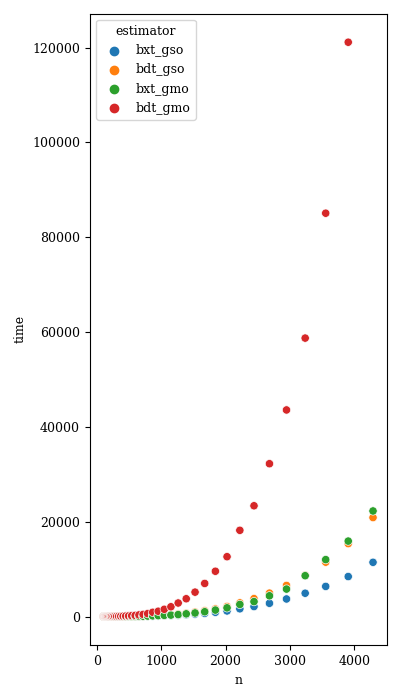
\includegraphics[width=\textwidth]{
            run_experiments/empirical_complexity/time_vs_n_artificial_data.png
        }
        \caption{Training durations in seconds versus the the number of samples and features.}
    \end{subfigure}
    \begin{subfigure}{0.5\textwidth}
        \includegraphics[width=\textwidth]{
            run_experiments/empirical_complexity/%
            time_vs_n_artificial_data_loglog.png
        }
        \caption{Logarithm of the training durations in seconds versus the logarithm of the number of samples and features.}
    \end{subfigure}
    \caption{
        Empirical time complexity estimation of the proposed bipartite tree
        algorithms. bxt stands for bipartite ExtraTree, bdt for a bipartite decision tree using the greedy split search procedure. Independent two sample t-tests comparing the slope estimates in (b) reveal that the time complexity of bdt\_gso is highly significantly lower than bdt\_gmo (p-value $< 10^{-37}$) and also that bxt\_gso significantly exibits lower complexity than bxt\_gmo (p-value $< 10^{-19}$). Those values
        corroborate the theoretical estimates from Section \ref{sec:complexity_analysis}.
    }
    \label{fig:empirical_complexity}
\end{figure}

\subsection{Comparison between GSO models}

To access the impact of global single-output optimizations in bipartite decision tree growing, we compare three slightly different training methods for BXT and BRF models.

\begin{itemize}
    \item \textbf{ngso}: Naive global single output implementation (Section \ref{});
    \item \textbf{ngsous}: Naive global single output implementation with undersampling of the non-interacting pairs to yield a balanced training set (Section \ref{});
    \item \textbf{gso}: Optimized implementation of global single output trees (Section \ref{}).
\end{itemize}

While no significant divergence was measured among the GSO models using the entirety of the training data, undersampling revealed to significantly degrade the predictive performance of both forests in terms of AUPR and MCC (Figure \ref{fig:cdd_gso_models}), eventhough it is arguably the most common procedure when dealing with this kind of data \cite{}.

On the other hand, AUROC is significantly improved by the undersampling procedure, which is most likely an artifact of the highly imbalanced nature of the present data, as explained as follows. The models grown on the undersampled datasets are naturally the most likely to assign positive labels to new interactions in general, improving TPR at the expense of also increasing FPR. However, since negative labels greatly outnumbers positive labels in the test sets of our current scenario, an increase in FPR impacts a much larger number of predictions than the same increase in TPR. In spite of that, AUROC equally treats TPR and FPR, so that the impact of a high FPR is underestimated. As such, AUROC results could be deemed as unrepresentative of model performance in this setup.

\begin{figure*}
    \centering
    \begin{subfigure}{0.32\textwidth}
        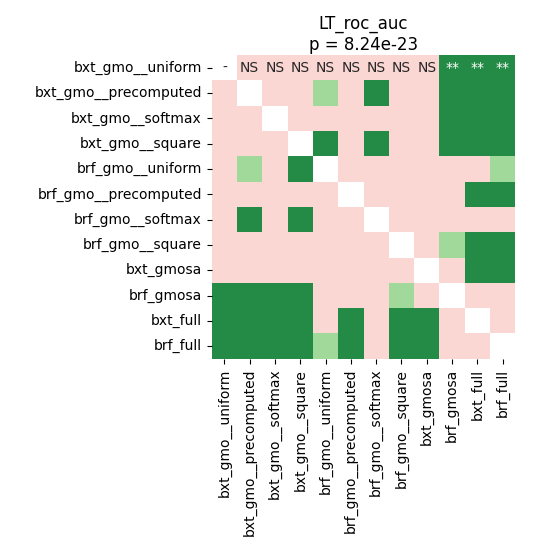
\includegraphics[width=\textwidth]{
            run_experiments/gso_optimization/figures/%
            estimator_name/enzymes__LT_roc_auc.png
        }
    \end{subfigure}
    \begin{subfigure}{0.32\textwidth}
        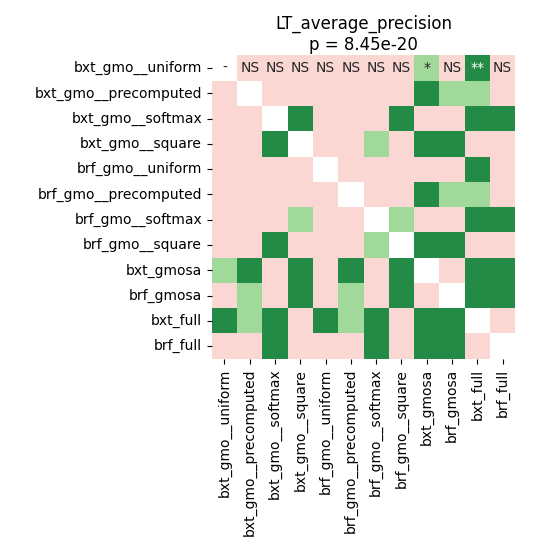
\includegraphics[width=\textwidth]{
            run_experiments/gso_optimization/figures/%
            estimator_name/enzymes__LT_average_precision.png
        }
    \end{subfigure}
    \begin{subfigure}{0.32\textwidth}
        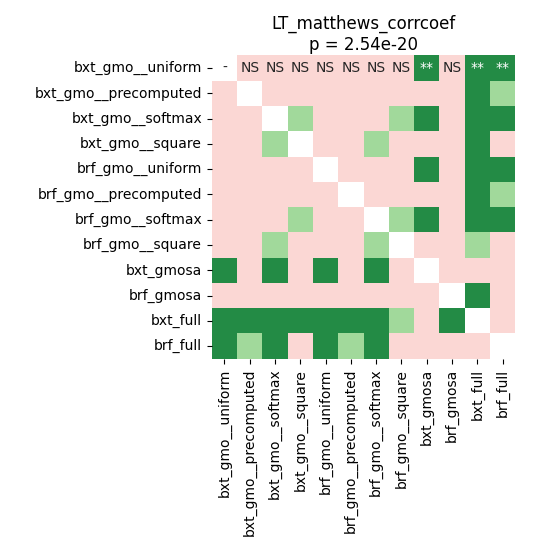
\includegraphics[width=\textwidth]{
            run_experiments/gso_optimization/figures/%
            estimator_name/enzymes__LT_matthews_corrcoef.png
        }
    \end{subfigure}

    \begin{subfigure}{0.32\textwidth}
        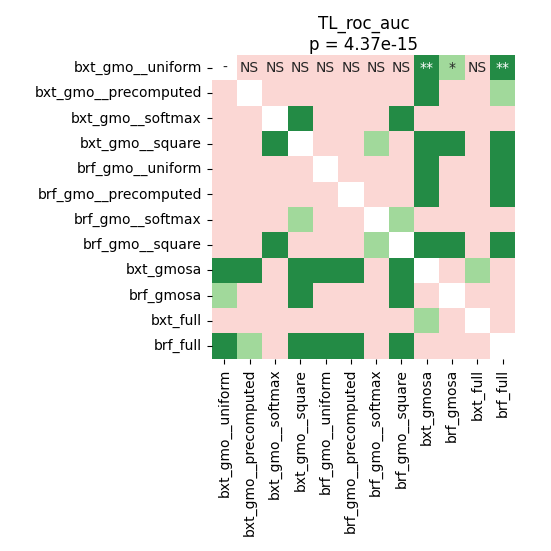
\includegraphics[width=\textwidth]{
            run_experiments/gso_optimization/figures/%
            estimator_name/enzymes__TL_roc_auc.png
        }
    \end{subfigure}
    \begin{subfigure}{0.32\textwidth}
        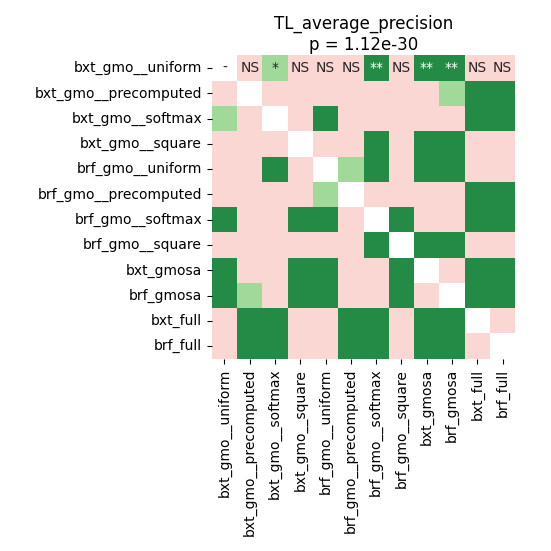
\includegraphics[width=\textwidth]{
            run_experiments/gso_optimization/figures/%
            estimator_name/enzymes__TL_average_precision.png
        }
    \end{subfigure}
    \begin{subfigure}{0.32\textwidth}
        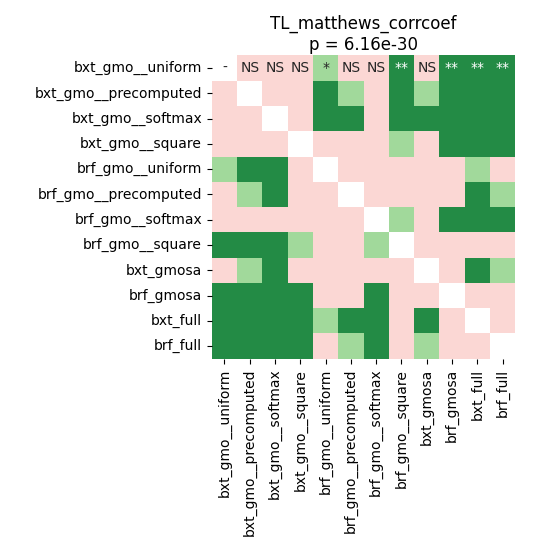
\includegraphics[width=\textwidth]{
            run_experiments/gso_optimization/figures/%
            estimator_name/enzymes__TL_matthews_corrcoef.png
        }
    \end{subfigure}

    \begin{subfigure}{0.32\textwidth}
        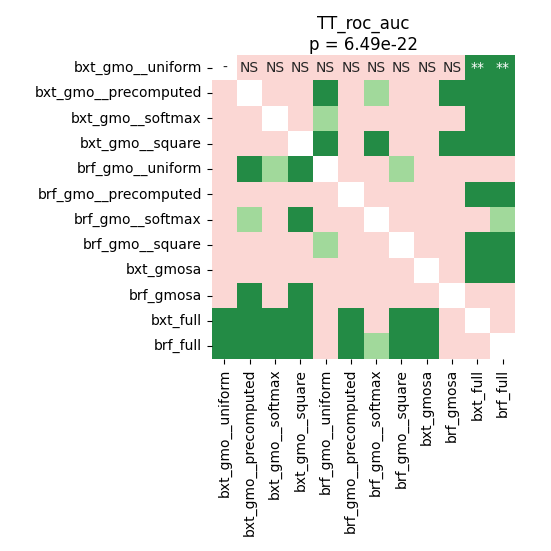
\includegraphics[width=\textwidth]{
            run_experiments/gso_optimization/figures/%
            estimator_name/enzymes__TT_roc_auc.png
        }
    \end{subfigure}
    \begin{subfigure}{0.32\textwidth}
        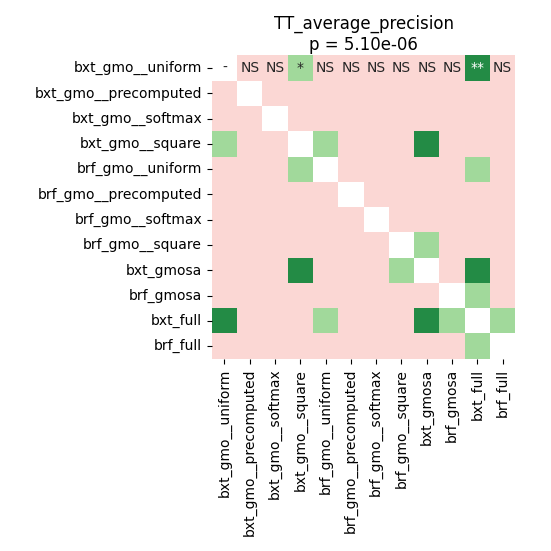
\includegraphics[width=\textwidth]{
            run_experiments/gso_optimization/figures/%
            estimator_name/enzymes__TT_average_precision.png
        }
    \end{subfigure}
    \begin{subfigure}{0.32\textwidth}
        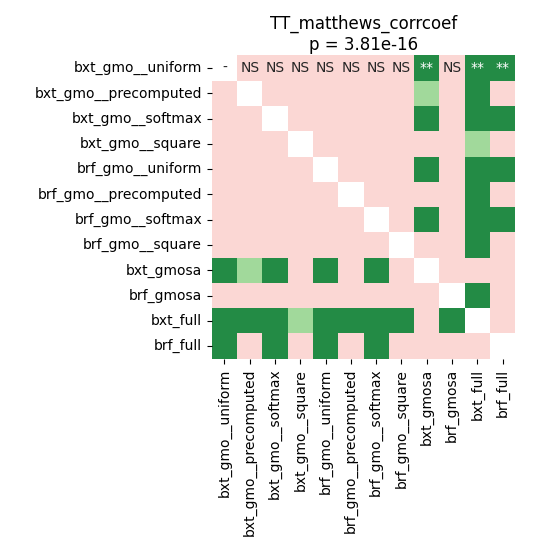
\includegraphics[width=\textwidth]{
            run_experiments/gso_optimization/figures/%
            estimator_name/enzymes__TT_matthews_corrcoef.png
        }
    \end{subfigure}
    \caption{Comparison between GSO models on the Enzymes dataset.}
    \label{fig:box_gso_models_enzymes}
\end{figure*}


\begin{figure*}
    \centering
    \begin{subfigure}{0.32\textwidth}
        \includegraphics[width=\textwidth]{
            run_experiments/gso_optimization/post_hoc/%
            all_datasets__cdd__LT_roc_auc.png
        }
    \end{subfigure}
    \begin{subfigure}{0.32\textwidth}
        \includegraphics[width=\textwidth]{
            run_experiments/gso_optimization/post_hoc/%
            all_datasets__cdd__LT_average_precision.png
        }
    \end{subfigure}
    \begin{subfigure}{0.32\textwidth}
        \includegraphics[width=\textwidth]{
            run_experiments/gso_optimization/post_hoc/%
            all_datasets__cdd__LT_matthews_corrcoef.png
        }
    \end{subfigure}

    \begin{subfigure}{0.32\textwidth}
        \includegraphics[width=\textwidth]{
            run_experiments/gso_optimization/post_hoc/%
            all_datasets__cdd__TL_roc_auc.png
        }
    \end{subfigure}
    \begin{subfigure}{0.32\textwidth}
        \includegraphics[width=\textwidth]{
            run_experiments/gso_optimization/post_hoc/%
            all_datasets__cdd__TL_average_precision.png
        }
    \end{subfigure}
    \begin{subfigure}{0.32\textwidth}
        \includegraphics[width=\textwidth]{
            run_experiments/gso_optimization/post_hoc/%
            all_datasets__cdd__TL_matthews_corrcoef.png
        }
    \end{subfigure}

    \begin{subfigure}{0.32\textwidth}
        \includegraphics[width=\textwidth]{
            run_experiments/gso_optimization/post_hoc/%
            all_datasets__cdd__TT_roc_auc.png
        }
    \end{subfigure}
    \begin{subfigure}{0.32\textwidth}
        \includegraphics[width=\textwidth]{
            run_experiments/gso_optimization/post_hoc/%
            all_datasets__cdd__TT_average_precision.png
        }
    \end{subfigure}
    \begin{subfigure}{0.32\textwidth}
        \includegraphics[width=\textwidth]{
            run_experiments/gso_optimization/post_hoc/%
            all_datasets__cdd__TT_matthews_corrcoef.png
        }
    \end{subfigure}
    \caption{Percentile score rankings for each global single output strategy.}
    \label{fig:cdd_gso_models}
\end{figure*}

% TODO: talk about pairwise CV

When comparing training times, the common choice for undersampling in previous works is justified, as an expressive reduction of training time is observed for both forests (Table \ref{}) relative to naive GSO training. Nevertheless, it is remarkable that the optimized implementation of GSO forests achieves similar training times in comparison to undersampled GSO without the AUPR and MCC burden of undersampling, keeping the higher scores resulting from employing the entirety of the dataset. For larger and less imbalanced datasets, the optimized implementation of GSO forests is expected to be even more advantageous, in agreement with the theoretical time complexity analysis (Section \ref{}).

%\begin{table}[h]
%    \input{
%        figures/run_experiments/gso_optimization/%
%        latex_tables/fit.tex
%    }
%\end{table}

In conclusion, the proposed approach confidently enables the use of the entire training data in a much shorter time frame than naive implementations without the need for data undersampling, which is statistically expected to yield better prediction scores for forest predictors.


\subsection{Comparison between GMO prediction weights}

In order to compare the different prediction weighting strategies (see Section \ref{}), a BXT and a BRF model were built for every option. The minimum rows per leaf and minimum columns per leaf were both set to 5, ensuring a minimum number of co-leaf samples of each sample domain to be taken into consideration in a weighted-neighbors fashion during evaluation (Section \ref{}).

As shown by Figure \ref{} and Table \ref{}, BXT models show an overall superior performance in comparison to BRF models, with each BXT model scoring significantly higher than its BRF counterpart with the same prediction weights. Furthermore, the weighted GMO predictions seem to prevail relative to the leaf-wise prototype GMOSA (Section \ref{}). Specifically, bxt\_square significantly outperforms all other bipartite forests except for bxt\_precomputed, both in terms of AUROC and average precision (AUPR) in the TT sets (Figure \ref{}).

\begin{figure*}
    \centering
    \begin{subfigure}{0.32\textwidth}
        \includegraphics[width=\textwidth]{
            run_experiments/prediction_weights/post_hoc/%
            all_datasets__cdd__LT_roc_auc.png
        }
    \end{subfigure}
    \begin{subfigure}{0.32\textwidth}
        \includegraphics[width=\textwidth]{
            run_experiments/prediction_weights/post_hoc/%
            all_datasets__cdd__LT_average_precision.png
        }
    \end{subfigure}
    \begin{subfigure}{0.32\textwidth}
        \includegraphics[width=\textwidth]{
            run_experiments/prediction_weights/post_hoc/%
            all_datasets__cdd__LT_matthews_corrcoef.png
        }
    \end{subfigure}

    \begin{subfigure}{0.32\textwidth}
        \includegraphics[width=\textwidth]{
            run_experiments/prediction_weights/post_hoc/%
            all_datasets__cdd__TL_roc_auc.png
        }
    \end{subfigure}
    \begin{subfigure}{0.32\textwidth}
        \includegraphics[width=\textwidth]{
            run_experiments/prediction_weights/post_hoc/%
            all_datasets__cdd__TL_average_precision.png
        }
    \end{subfigure}
    \begin{subfigure}{0.32\textwidth}
        \includegraphics[width=\textwidth]{
            run_experiments/prediction_weights/post_hoc/%
            all_datasets__cdd__TL_matthews_corrcoef.png
        }
    \end{subfigure}

    \begin{subfigure}{0.32\textwidth}
        \includegraphics[width=\textwidth]{
            run_experiments/prediction_weights/post_hoc/%
            all_datasets__cdd__TT_roc_auc.png
        }
    \end{subfigure}
    \begin{subfigure}{0.32\textwidth}
        \includegraphics[width=\textwidth]{
            run_experiments/prediction_weights/post_hoc/%
            all_datasets__cdd__TT_average_precision.png
        }
    \end{subfigure}
    \begin{subfigure}{0.32\textwidth}
        \includegraphics[width=\textwidth]{
            run_experiments/prediction_weights/post_hoc/%
            all_datasets__cdd__TT_matthews_corrcoef.png
        }
    \end{subfigure}
    \caption{Percentile score rankings for each prediction weighting strategy.}
    \label{fig:pred_weights}
\end{figure*}

% contribution: GMO models

Hence, the bxt\_square model was selected for the downstream analyses, keeping 5 by 5 as the minimum leaf partition size. While GMOSA will also be further investigated, the leaf size constraint will be dropped, generating fully grown trees for this strategy.


\subsection{Comparison between adaptation strategies}

Still restricted to forest estimators, we compare each of the described approaches for adapting models to bipartite data (Section \ref{}). To avoid differences in random sampling when using the naive GSO adapter versus the natively bipartite GSO tree, no bootstraping was applied to any forest, providing all trees with the whole training samples space. To still ensure randomization in random forest estimators, the maximum features parameter was set to $0.5$, meaning that each tree in a random forest was trained on a random subset of half the features from each sample domain. Due to implementation details, this means the naive GSO forests will sample features slightly differently: they will pick half the features from the whole feature space combined, while the natively bipartite GSO forests will ensure half the features from each sample domain is selected. This is not expected to have a significant impact on the results, given that the total number of features is especially high in the present scenario, where similarity matrices are being employed. 

All forests were composed of 100 tree estimators and were fully grown, with the exception of the GMO models, whose leaf sizes were limited to a minimum of 5 by 5 samples (at least 5 samples from each domain) in order to take advantage of neighborhood weighting (which was set to the squared similarities, see Section \ref{}).

In all of the evaluated scenarios, a BXT model was ranked the best. In both TT-MCC and TL-AP, the BRF models and bxt\_gmo were significantly surpassed by the remaining BXT forests. In TL-MCC, bxt\_lso significantly outperformed all the other models. Given that this test-set provides the greatest intersection with the training set, due to the overall higher number of column samples in the datasets we used, we suggest that the LSO model could be better at taking advantage of already seen information from a sample domain, since a forest is grown separately for each row and column. From another perspective, this effect could be regarded as a form of overfitting. This hypothesis is further supported by the fact that both GMO models, which were the only forests subject to a minimum leaf size constraint and thus less prone, in theory, to overfitting, were the most frequently outperformed models in the TL-MCC and TL-AP.

Contrastingly, both GMO models were consistently the best performing models in all AUROC settings, which is commonly assumed to be a less indicative metric in highly unbalanced classification contexts such as the present one \cite{}. This could be explained by a bias towards the majority class, possibly caused by the averaging of the larger leaves employed in this methods. %FIXME: actually, a bias towards minority class

\begin{figure*}
    \centering
    \begin{subfigure}{0.32\textwidth}
        \includegraphics[width=\textwidth]{
            run_experiments/bipartite_approaches/post_hoc/%
            all_datasets__cdd__LT_roc_auc.png
        }
    \end{subfigure}
    \begin{subfigure}{0.32\textwidth}
        \includegraphics[width=\textwidth]{
            run_experiments/bipartite_approaches/post_hoc/%
            all_datasets__cdd__LT_average_precision.png
        }
    \end{subfigure}
    \begin{subfigure}{0.32\textwidth}
        \includegraphics[width=\textwidth]{
            run_experiments/bipartite_approaches/post_hoc/%
            all_datasets__cdd__LT_matthews_corrcoef.png
        }
    \end{subfigure}

    \begin{subfigure}{0.32\textwidth}
        \includegraphics[width=\textwidth]{
            run_experiments/bipartite_approaches/post_hoc/%
            all_datasets__cdd__TL_roc_auc.png
        }
    \end{subfigure}
    \begin{subfigure}{0.32\textwidth}
        \includegraphics[width=\textwidth]{
            run_experiments/bipartite_approaches/post_hoc/%
            all_datasets__cdd__TL_average_precision.png
        }
    \end{subfigure}
    \begin{subfigure}{0.32\textwidth}
        \includegraphics[width=\textwidth]{
            run_experiments/bipartite_approaches/post_hoc/%
            all_datasets__cdd__TL_matthews_corrcoef.png
        }
    \end{subfigure}

    \begin{subfigure}{0.32\textwidth}
        \includegraphics[width=\textwidth]{
            run_experiments/bipartite_approaches/post_hoc/%
            all_datasets__cdd__TT_roc_auc.png
        }
    \end{subfigure}
    \begin{subfigure}{0.32\textwidth}
        \includegraphics[width=\textwidth]{
            run_experiments/bipartite_approaches/post_hoc/%
            all_datasets__cdd__TT_average_precision.png
        }
    \end{subfigure}
    \begin{subfigure}{0.32\textwidth}
        \includegraphics[width=\textwidth]{
            run_experiments/bipartite_approaches/post_hoc/%
            all_datasets__cdd__TT_matthews_corrcoef.png
        }
    \end{subfigure}
    \caption{Percentile score rankings for each bipartite adaptation approach.}
    \label{fig:cdd_adapters}
\end{figure*}

\subsection{Effect of interaction matrix reconstruction}

It was previously suggested that employing logistic matrix factorization to create a denser representation of the interaction matrix and using this representation as the training data for a BXT forest could improve their performance on DTI datasets \cite{Pliakos_2020}. To test this hypothesis, we compare the bipartite forests cross-validation scores with and without the interaction matrix reconstruction step. As done by \cite{Pliakos_2020}, the reconstruction step was performed using neighborhood-regularized logistic matrix factorization (NRLMF)\cite{}. The results are shown in Figure \ref{fig:cdd_reconstruction}.

To select hyperparameters for the NRLMF algorithm, we performed a randomized search in which 100 different combinations of hyperparameters were evaluated in terms of their resulting mean squared error over a (nested) bipartite 5-fold diagnonal cross-validation. The best combination found in the inner CV loop was then used to reconstruct the interaction matrix of each outer CV fold, and the resulting matrices were used as the training data for the bipartite forests. Note that a single forest was built by outer CV fold, so that the NRLMF hyperparameter seach was performed independently to the downstream forest performance. The hyperparameters \texttt{lambda\_rows}, \texttt{lambda\_cols}, \texttt{alpha\_cols}, \texttt{alpha\_cols}, and \texttt{learning\_rate} were all independently sampled from a log-uniform distribution bounded by $\frac{1}{4}$ and $2$. the number of latent vector components were set to be equal among noth axes, and chosen between 50 and 100. The number of neighbors was randomly selected as 3, 5 or 10 in each iteration, and the maximum number of optimization steps was always set to 100.

The results are shown in Figure \ref{fig:cdd_reconstruction}.

In accordance to the previous findings of \cite{Pliakos_2020}, the models with output space reconstruction either show significantly higher AUROC and AUPR or generated inconclusive results regarding those metrics when compared to the models without the reconstruction by NRLMF.

Surprisingly, however, the MCC results tend to favor the opposite conclusion, with the models without reconstruction showing higher MCC scores in most cases.

% TODO: remake the following explanation after displaying the rank boxplots

A first explanation could be that the NRLMF hyperparameter search was not exhaustive enough, and that a better combination of hyperparameters could have been found. However, we later show in section \ref{} that the NRLMF model alone displays competitive performance, disfavoring such hypothesis of underfitting.

We also notice that \cite{Liu_2017} performs bipartite cross-validation in unusual fashion, by replacing with zeros the positive labels of pairs assigned to the test set but still using them to train the model. Albeit test labels are masked, each model thus still receives all available samples during training, and we hypothesize that unsupervised information from the test set could possibly still be exploited during training. For instance, estimating the sample density of the feature space could provide an importance score, a weight factor, for each sample, in order to favor correct predictions of denser clusters and undermine outliers. Wether and how this or similar mechanisms are explored by the NRLMF algorithm is out of the scope of this work, but we discourage the use of such CV strategy and point it as a possible reason for the higher NRLMF scores observed by previous authors \cite{Pliakos_2020;Liu_2017}.

% (False, they also used nested CV) The authors of \cite{Pliakos_2020} also do not clearly specify the could have employed the reconstruction step before splitting the data into the cross-validation folds, in which case the observed performance improvement could be attributed to indirect data leakage, where the labels used to train the downstream forest estimator were generated from neighbor samples that are possibly in the test sets.

\begin{figure*}
    \centering
    \begin{subfigure}{0.32\textwidth}
        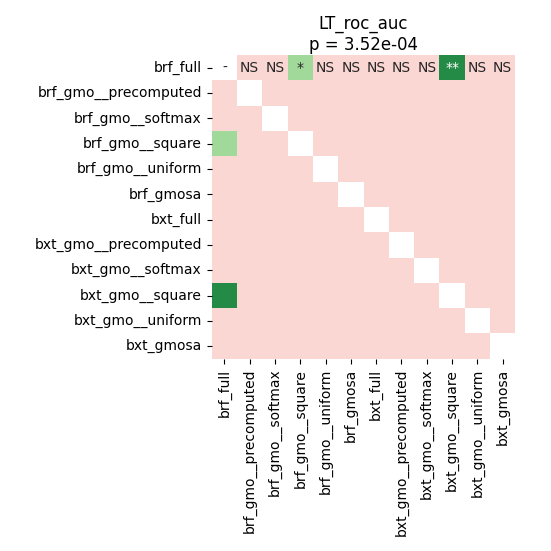
\includegraphics[width=\textwidth]{
            run_experiments/y_reconstruction/figures/%
            estimator_name/all_datasets__LT_roc_auc.png
        }
    \end{subfigure}
    \begin{subfigure}{0.32\textwidth}
        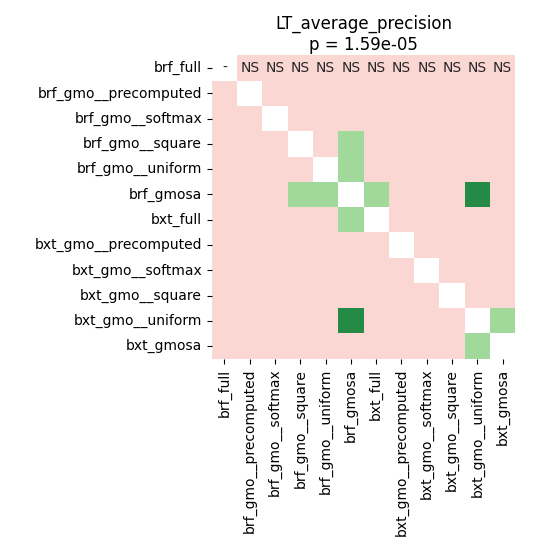
\includegraphics[width=\textwidth]{
            run_experiments/y_reconstruction/figures/%
            estimator_name/all_datasets__LT_average_precision.png
        }
    \end{subfigure}
    \begin{subfigure}{0.32\textwidth}
        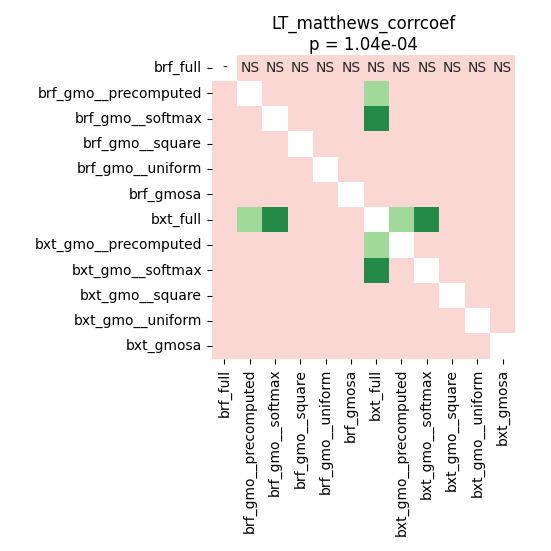
\includegraphics[width=\textwidth]{
            run_experiments/y_reconstruction/figures/%
            estimator_name/all_datasets__LT_matthews_corrcoef.png
        }
    \end{subfigure}

    \begin{subfigure}{0.32\textwidth}
        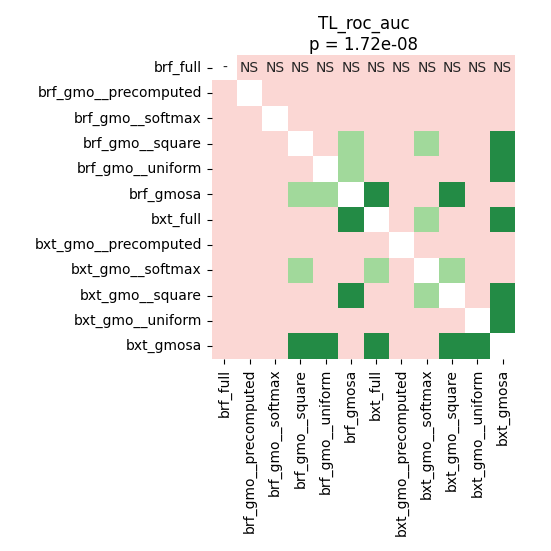
\includegraphics[width=\textwidth]{
            run_experiments/y_reconstruction/figures/%
            estimator_name/all_datasets__TL_roc_auc.png
        }
    \end{subfigure}
    \begin{subfigure}{0.32\textwidth}
        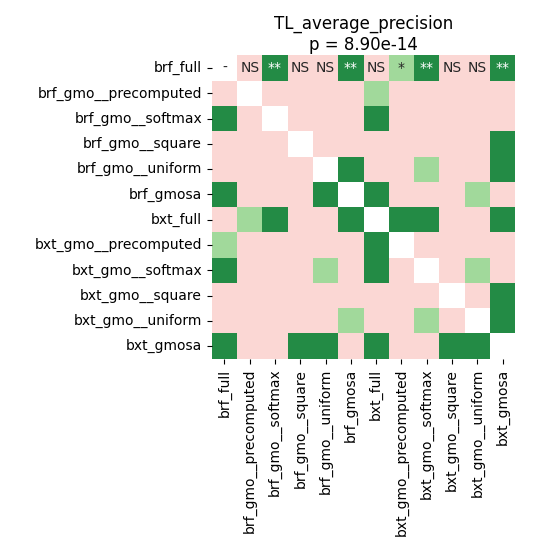
\includegraphics[width=\textwidth]{
            run_experiments/y_reconstruction/figures/%
            estimator_name/all_datasets__TL_average_precision.png
        }
    \end{subfigure}
    \begin{subfigure}{0.32\textwidth}
        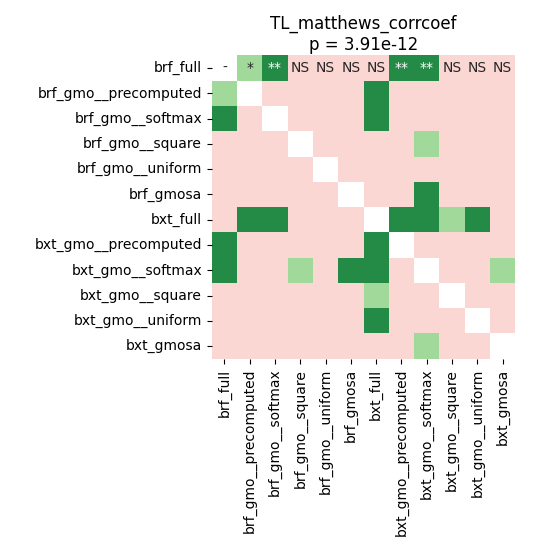
\includegraphics[width=\textwidth]{
            run_experiments/y_reconstruction/figures/%
            estimator_name/all_datasets__TL_matthews_corrcoef.png
        }
    \end{subfigure}

    \begin{subfigure}{0.32\textwidth}
        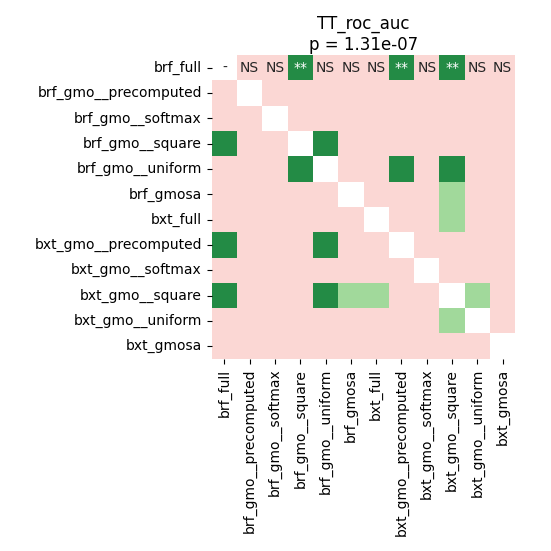
\includegraphics[width=\textwidth]{
            run_experiments/y_reconstruction/figures/%
            estimator_name/all_datasets__TT_roc_auc.png
        }
    \end{subfigure}
    \begin{subfigure}{0.32\textwidth}
        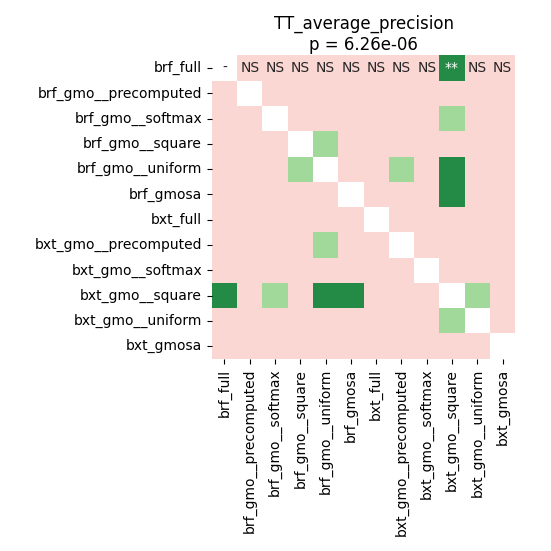
\includegraphics[width=\textwidth]{
            run_experiments/y_reconstruction/figures/%
            estimator_name/all_datasets__TT_average_precision.png
        }
    \end{subfigure}
    \begin{subfigure}{0.32\textwidth}
        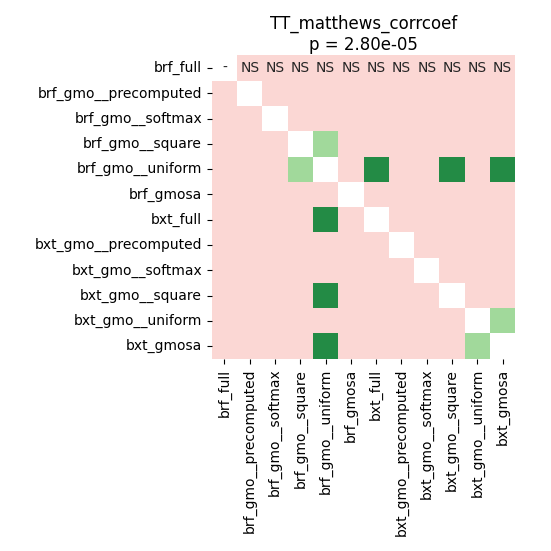
\includegraphics[width=\textwidth]{
            run_experiments/y_reconstruction/figures/%
            estimator_name/all_datasets__TT_matthews_corrcoef.png
        }
    \end{subfigure}
    \caption{Comparison of scores for the bipartite forests with and without output space reconstruction on the enzymes dataset.}
    \label{fig:box_y_reconstruction}
\end{figure*}

% \begin{table}[h]
%     \input{figures/run_experiments/y_reconstruction/latex_tables/TT.tex}
% \end{table}


\subsection{Comparison with previous works}

In this section we employ several algorithms previously described in the literature, all of which were reimplemented and had their performance measured on the four DTI prediction datasets according to this study's evaluation framework (Section \ref{}).

The algorithms being considered in this section are listed below, and their scoring results are shown in Figure \ref{fig:cdd_literature} and Table \ref{}. To further explore the potential of bipartite forests, all forests evaluated in this section were composed of 1000 trees, as opposed to the 100 trees used in the previous experiments.

\begin{itemize}
    \item NRLMF \cite{Liu_2017}
    \item BLM-NII 
    % TODO
\end{itemize}

Regarding the AUROC metric, bxt\_gmosa\_nrlmf, bxt\_gso\_nrlmf and nrlmf are consistently the three highest ranked models in all three testing settings, with both bxt\_gmosa\_nrlmf and bxt\_gso\_nrlmf significantly outperforming BLM-NII-SVM, BLM-NII-RLS, and DTHybrid.
Additionally, DNILMF was outperformed by bxt\_gmosa\_nrlmf and bxt\_gso\_nrlmf in the TL and LT settings, and by bxt\_gmosa\_nrlmf in the TT setting.

Both in the LT and TT settings, the bipartite forests without matrix reconstruction (bxt\_gmosa and bxt\_gso) showed no significant difference in performance when compared to their counterparts employing interaction matrix reconstruction by NRLMF (bxt\_gmosa\_nrlmf and bxt\_gso\_nrlmf, respectively), contrary to the results on the TL testing configuration, where matrix reconstruction was shown to be significantly beneficial.
A possible explanation relies on the fact that the TL test set has the higher intersection with the training data in our specific scenario, since in the four datasets considered the drug molecules outnumber the protein targets by considerable margins (see Table \ref{tab:datasets}).
That said, NRLMF fundamentally relies on the label information of a small neighborhood of each sample to infer interactions and, as such, this result may suggest that the benefit of the matrix factorization step is elevated in cases where the test set is similar to the training set, and could be specifically useful in drug repurposing scenarios rather than in drug discovery. On the other hand, overfitting may arise as a potential concern when new drugs and new targets are of the main interest.

Additionally, one must recall we are using larger forests in comparison to the previous section, which may render the matrix factorization step less relevant.
This is further supported by the fact that the NRLMF model itself could not significantly outperform bxt\_gso in the LT\_roc\_auc setting, bxt\_gmosa in the TL\_roc\_auc setting and also could not outperform either forest in the TT\_roc\_auc setting (Figure \ref{fig:cdd_literature}), not ruling out the explanation that the tree ensemble itself is sufficient to encompass neighborhood information.

When the average precision metric is considered, the reconstruction step is again regarded unbeneficial, with no significant difference in employing it versus using the bipartite forest alone. Interestingly, all BXT forests perform significantly better than all other methods in the TL\_average\_precision setting, even than the matrix factorization techniques NRLMF and DNILMF (Figure \ref{fig:cdd_literature}). NRLMF, DNILMF and lmorls were the only methods not proven significantly inferior to the BXT in the remaining average precision settings. 

The superiority of DNILMF with respect to NRLMF as claimed by its authors \cite{} was not observed in our experiments, with NRLMF even proven significantly superior to DNILMF in the TL\_roc\_auc and LT\_roc\_auc settings (Figure \ref{fig:cdd_literature}).

With respect to the MCC metric, the bxt\_gmosa and bxt\_gso stand out as the best performing models, significantly outperforming all the other models in TL\_mcc, all but bxt\_gmosa\_nrlmf in LT\_mcc, and all but bxt\_gmosa\_nrlmf and bxt\_gso\_nrlmf in the TT setting.

However, this result is likely affected by the classification threshold choice, since this is the only metric we used that is threshold-dependent. Since we chose this threshold as the probability of interaction in each training set (the average of all binary values of $y$), the MCC metric will favor well calibrated models, i.e. whose predicted probabilities are close to the measured propabilities.  % TODO: define better and cite
As such, this result mainly indicates better calibration of the BXT models out of the box. Conversely, the other models may benefit from calibration techniques such as Platt scaling \cite{} or isotonic regression \cite{}, with BLM models being especially underperformant regarding MCC.

Overall, bxt\_gso and bxt\_gmosa are the most consistently higher ranked models among the algorithms we tested. Remarkably, we demonstrate in sections \ref{sec:complexity_analysis} and \ref{sec:empirical_complexity} that our optimized GSO forests are considerably faster to train than the GMO forests proposed by \cite{Pliakos_2018}, even if no statistically significant decrease in performance is observed. This time complexity superiority enables forest estimators to tackle much larger bipartite datasets than was possible with the current bipartite trees, and points native GSO bipartite forests as a strong candidate to be further studied across similar learning scenarios in the future.

\begin{figure*}
    \centering
    \begin{subfigure}{0.32\textwidth}
        \includegraphics[width=\textwidth]{
            run_experiments/literature_models/post_hoc/%
            all_datasets__cdd__LT_roc_auc.png
        }
    \end{subfigure}
    \begin{subfigure}{0.32\textwidth}
        \includegraphics[width=\textwidth]{
            run_experiments/literature_models/post_hoc/%
            all_datasets__cdd__LT_average_precision.png
        }
    \end{subfigure}
    \begin{subfigure}{0.32\textwidth}
        \includegraphics[width=\textwidth]{
            run_experiments/literature_models/post_hoc/%
            all_datasets__cdd__LT_matthews_corrcoef.png
        }
    \end{subfigure}

    \begin{subfigure}{0.32\textwidth}
        \includegraphics[width=\textwidth]{
            run_experiments/literature_models/post_hoc/%
            all_datasets__cdd__TL_roc_auc.png
        }
    \end{subfigure}
    \begin{subfigure}{0.32\textwidth}
        \includegraphics[width=\textwidth]{
            run_experiments/literature_models/post_hoc/%
            all_datasets__cdd__TL_average_precision.png
        }
    \end{subfigure}
    \begin{subfigure}{0.32\textwidth}
        \includegraphics[width=\textwidth]{
            run_experiments/literature_models/post_hoc/%
            all_datasets__cdd__TL_matthews_corrcoef.png
        }
    \end{subfigure}

    \begin{subfigure}{0.32\textwidth}
        \includegraphics[width=\textwidth]{
            run_experiments/literature_models/post_hoc/%
            all_datasets__cdd__TT_roc_auc.png
        }
    \end{subfigure}
    \begin{subfigure}{0.32\textwidth}
        \includegraphics[width=\textwidth]{
            run_experiments/literature_models/post_hoc/%
            all_datasets__cdd__TT_average_precision.png
        }
    \end{subfigure}
    \begin{subfigure}{0.32\textwidth}
        \includegraphics[width=\textwidth]{
            run_experiments/literature_models/post_hoc/%
            all_datasets__cdd__TT_matthews_corrcoef.png
        }
    \end{subfigure}
    \caption{Percentile score rankings for several literature models.}
    \label{fig:cdd_literature}
\end{figure*}


% linear models underfitted. previous good results in TL an LT are likely partial data leakage due to network feature extraction

% even in TT, data leakage could occur if cv is performed by masking positives

% partial conclusions:
% no need for matrix factorization step
% calibration is needed
% gso is competing in the top, even if theorically faster
% extratrees are better than rf for these datasets

\subsection{Drug-Target affinity prediction}

In this section, we evaluate bipartite forests performance in a bipartite regression dataset, comparing them to state of the art deep neural networks.

\begin{itemize}
    \item deep\_dta\_raw: Uses convolutional layers to encode raw amino acid sequences and SMILES strings of drug molecules. DeepDTA \cite{Ozturk_2018}
    \item transformer\_raw: DNN employing transformer modules to embedd the raw amino acid sequence of target proteins and SMILES string of drug molecules. Parameters were based on MolTrans \cite{}
\end{itemize}

The bxt\_gmosa model \cite{Pliakos_2020} significantly outperforms both neural networks and brf\_gso in all scenarios. bxt\_gso also outperforms the neural networks and brf\_gso in the TT setting, and score significantly higher than brf\_gso and transformer\_raw in the remaining configurations. Most impressively, the forest models take considerably less time to train than the neural networks given the experimental setup, as shown by Figure \ref{fig:davis_mse}, with the bxt\_gso still displaying highly competitive performance despite providing sensible gains in time complexity in comparison to the GMO forests and a naive GSO implementation (see sections \ref{sec:complexity_analysis} and \ref{sec:empirical_complexity}).

This result points bipartite ExtraTree ensembles as state-of-the-art regression models in drug-target affinity prediction tasks, with highly competitive improvements in training efficiency.

% TODO: comment on GPU possible improvements

\begin{figure*}
    \centering
    \begin{subfigure}{0.24\textwidth}
        \includegraphics[width=\textwidth]{
            run_experiments/neural_nets/post_hoc/%
            davis__boxplot__LT_neg_mean_squared_error.png
        }
        \caption{Negative mean squared error on the LT test set.}
    \end{subfigure}
    \begin{subfigure}{0.24\textwidth}
        \includegraphics[width=\textwidth]{
            run_experiments/neural_nets/post_hoc/%
            davis__boxplot__TL_neg_mean_squared_error.png
        }
        \caption{Negative mean squared error on the TL test set.}
    \end{subfigure}
    \begin{subfigure}{0.24\textwidth}
        \includegraphics[width=\textwidth]{
            run_experiments/neural_nets/post_hoc/%
            davis__boxplot__TT_neg_mean_squared_error.png
        }
        \caption{Negative mean squared error on the TT test set.}
    \end{subfigure}
    \begin{subfigure}{0.24\textwidth}
        \includegraphics[width=\textwidth]{
            run_experiments/neural_nets/post_hoc/%
            davis__boxplot__fit_time.png
        }
        \caption{Training duration in seconds.}
    \end{subfigure}

    \begin{subfigure}{0.24\textwidth}
        \includegraphics[width=\textwidth]{
            run_experiments/neural_nets/post_hoc/%
            davis__boxplot__LT_r2.png
        }
        \caption{$R^2$ score on the LT test set.}
    \end{subfigure}
    \begin{subfigure}{0.24\textwidth}
        \includegraphics[width=\textwidth]{
            run_experiments/neural_nets/post_hoc/%
            davis__boxplot__TL_r2.png
        }
        \caption{$R^2$ score on the TL test set.}
    \end{subfigure}
    \begin{subfigure}{0.24\textwidth}
        \includegraphics[width=\textwidth]{
            run_experiments/neural_nets/post_hoc/%
            davis__boxplot__TT_r2.png
        }
        \caption{$R^2$ score on the TT test set.}
    \end{subfigure}
    \begin{subfigure}{0.24\textwidth}
        \includegraphics[width=\textwidth]{
            run_experiments/neural_nets/post_hoc/%
            davis__boxplot__score_time.png
        }
        \caption{Prediction duration in seconds.}
    \end{subfigure}

    \caption{Model performance on the DAVIS dataset.}
    \label{fig:davis_mse}
\end{figure*}


\subsection{Estimated impact of missing labels}


\section{Final remarks}

A new Biclustering Random Forest (BRF), and semi-supervised tree-ensembles models were proposed.

The BRF estimator obtained competitive scores against the original PBCT ensemble model eBICT, with nearly 0.1 higher AUROC median on completely new test sets, although not statistically significant.

Using only the splitting feature column to calculate impurity lead to poorer results and thus needs technique refinements for future analyses.

% \subsection{Next steps}
% prunning
% 
% datasets
% 
% boosting
% 
% monopartite to bipartite approximation
% 
% n-partite data